\documentclass[11pt]{article}

\usepackage{graphicx} % Required for inserting images
\graphicspath{ {./images/} }
\usepackage{subcaption}

\usepackage{biblatex}
\addbibresource{references.bib}

\usepackage{csquotes}
\usepackage{dirtytalk}

\usepackage{tikz}
\usetikzlibrary{arrows,intersections,calc}

\usepackage{pgfmath}

\usepackage{listings}
\usepackage{color}

\usepackage{geometry}
\geometry{margin=3cm}

\DeclareMathSymbol{*}{\mathbin}{symbols}{"01}

\definecolor{dkgreen}{rgb}{0,0.6,0}
\definecolor{gray}{rgb}{0.5,0.5,0.5}
\definecolor{mauve}{rgb}{0.58,0,0.82}

\lstset{frame=tb,
  language=[5.2]Lua,
  aboveskip=3mm,
  belowskip=3mm,
  showstringspaces=false,
  columns=flexible,
  basicstyle={\small\ttfamily},
  numbers=none,
  numberstyle=\tiny\color{dkgreen},
  keywordstyle=\color{blue},
  commentstyle=\color{gray},
  stringstyle=\color{mauve},
  breaklines=true,
  breakatwhitespace=true,
  tabsize=3
}

\renewcommand{\abstractname}{Executive Summary}

% \title{A three-dimensional rail shooter in PICO-8}
% \author{Harry Jackson}
% \date{September 2025}

\begin{document}
% \maketitle

\begin{titlepage}
   \begin{center}
       \vspace*{1cm}

       \huge
       \textbf{A three-dimensional rail shooter in PICO-8}

       \vspace{1.5cm}

       \large
       \textbf{Harry Jackson}

       \vspace{0.5cm}

       Supervised by Dr John Lapinskas

       \vfill
            
       A dissertation submitted to the University of Bristol in accordance
       with the requirements of the degree of Master of Science in
       the Faculty of Engineering.
            
       \vspace{0.8cm}
     
       
\includegraphics[width=0.4\textwidth]{university}

       \vspace{0.8cm}
            
       Department of Computer Science\\
       University of Bristol\\
       September 2025\\
            
   \end{center}
\end{titlepage}

\section*{Author's declaration}

\vspace{0.5cm}

I declare that the work in this dissertation was carried out in accordance with the
requirements of the University’s Regulations and Code of Practice for Research
Degree Programmes and that it has not been submitted for any other academic
award. Except where indicated by specific reference in the text, the work is the
candidate’s own work. Work done in collaboration with, or with the assistance of,
others, is indicated as such. Any views expressed in the dissertation are those of the
author.

\vspace{0.5cm}

Signed:


\includegraphics[width=0.8\textwidth]{signature}

Date: 2 September 2025

\newpage

\section*{Executive summary}

\vspace{0.5cm}

The rail shooter was one of the earliest attempts to bring video
games into the third-dimension - first through the use of pseudo-3D
scaling effects, and later through the use of real-time polygonal graphics.

This project seeks to explore this category of interactive software through a
modern implementation for PICO-8 - a ``fantasy console'' which replicates the
computational and data constraints of historical system hardware on which
developers typically eschewed polygonal rendering for simpler 2D effects.

We will attempt to develop a playable 3D rail shooter using a
blended approach to graphics rendering - using both sprite scaling techniques and
also a limited degree of real time polygonal rendering, to create satisfying
gameplay in both depth and rotation governed by appropriate real-time 3D systems.

\vspace{1.5cm}

\section*{Acknowledgements}

\vspace{0.5cm}

I would like to thank my supervisor Dr John Lapinskas for his advice and guidance
throughout the project.

\newpage

\tableofcontents

\newpage

\section{Introduction, aims, and objectives}

The following project is a software implementation of a rail shooter, simulating a 3D 
environment through the blended use of projected and scaled 2D sprites alongside
limited real time polygonal rendering.

Rail shooters were a staple of arcade and later home console video games in the 1980s and
1990s, spearheading technical innovations and helping to bring video games into the third
dimension. In such games, player move in a linear fashion through space with limited
spatial control, and engage in shooting gallery style gameplay against groups of enemies.

Our implementation, for the ``fantasy console'' PICO-8, will work within the constraints of
our chosen technology by replicating sprite scaling techniques used in implementations built
on similarly constrained technology, while pushing further to introduce a limited degree of
real-time polygonal rendering and exploring the potential of this approach for more complex
gameplay that allows players to explore 3D space through rotational strafing.

In the course of this project report I will:

\begin{itemize}
   \item introduce the rail shooter as a genre of interactive software through a brief history and gameplay taxonomy;
   \item introduce our chosen technology, the PICO-8 ``fantasy console'', and provide rationale for its selection;
   \item walk through the process of implementation, including initial paper and software prototyping, developed 3D 
   prototyping, and lastly our final implementation - discussing, along the way, relevant technical issues like 
   3D point projection, camera manipulation, and real time collision detection, as well as design decisions taken
   with respect for technical constraints, genre conventions, and qualitative and quantitative user testing;
   \item evaluate the work completed and sketch further work for future development of the project.
\end{itemize}

The project repository is available on GitHub at \url{https://github.com/hjx92/msc-project} and the game can
be played at \url{https://hjx92.github.io/msc-project/}.

If played on a gamepad, as intended, player inputs typically map in an intuitive fashion - the four D-pad inputs
will correspond to the D-pad of the gamepad, the two face buttons will map to the two primary face buttons of
the gamepad, and the start button will correspond to the start button of the gamepad.

If played on a keyboard, the arrow keys will correspond to the D-pad, the Z and X keys will correspond to
PICO-8's face buttons, and the Enter key will correspond to Start.

\section{Background and context}

\subsection{The rail shooter}\label{genre}

\subsubsection*{Historical outline}
The rail shooter was one of the first attempts to bring video games into the third dimension and sat at the cutting
edge of technical game development across the 1980s and much of the 1990s.

Early entries in the genre relied primarily
on sprite-scaling effects facilitated first by Sega's Super Scaler arcade board, and later (in more primitive form) by the publisher's
home consoles. \textit{Space Harrier}\cite{space_harrier}, which debuted on the Super Scaler board in 1985, demonstrated
the utility of this approach for fast paced action combat games, allowing players to enter a bizarre
fantasy sci-fi world in which an unnamed warrior levitates through space and blasts a variety of
enemy craft and alien creatures with a powerful energy gun. Meanwhile \textit{Hang-On} showcased the use of this technique
for games in the racing genre, simulating approaching sharp turns and rival motorcycles with an illusion
of 3D depth.

Both of these distinctive Super Scaler game genres - the rail shooter and the pseudo-3D
racer - would see continued development in the years to come with more sophisticated arcade board
technology that allowed developers to depict a greater number of sprites and apply more complex
transformations to them, such as real-time rotation. Of these later entries, \textit{After Burner} is the
most notable of the rail shooters, allowing players to take control of a supersonic fighter jet speeding
across the ocean, while \textit{Outrun} remains the most iconic of the Super Scaler driving games.

In 1993, Argonaut Software's acclaimed title \textit{Star Fox}\cite{star_fox} for the Super Nintendo Entertainment
System took the genre a step further with the integration of real-time polygonal graphics. Augmenting
the Super Nintendo's native hardware with the Super FX chip - an on-cartridge co-processor for graphics acceleration -
\textit{Star Fox} saw players traverse worlds with polygonal enemies and simple 3D world geometry,
engaging in the genre's staple aim-and-shoot gameplay while also adding a more involved navigational element that
sees players moving through gates throughout the level.

Sega's 1995 title \textit{Panzer Dragoon}\cite{panzer_dragoon}, launched for the Sega Saturn in Japan before 
the console's international rollout, brought richer texture-mapped 3D worlds and a celebrated orchestral
soundtrack by composer Yoshitaka Azuma, once again showcasing advances in home console technology - in this case, the
shift to less memory constrained disc-based media that could bear texture map information and extensive high quality
audio.

The genre reached its aesthetic apotheosis with \textit{Rez}\cite{rez} in 2001 for the Sega Dreamcast.
The game uses more pared back wireframe graphics to depict a hacker's infiltration of a computer system,
and exploits the scripted nature of the genre by synchronising gameplay to an intense electronic music soundtrack.

The game also made interesting design decisions as a response to the Dreamcast's antiquated
single-analogue input that continue to be felt on modern systems to which the game has been ported and
continues to be popular - most notably to the Xbox 360 as \textit{Rez HD}, and to the PlayStation 4,
PlayStation 5, and Oculus Quest as \textit{Rez Infinite} with new VR modes.

Although dedicated commercial rail shooters are now virtually extinct, the gameplay mechanics
do live on in sections of popular games where players lose free control of player movement
and engage in moving shooting galleries - a defining trait of the genre, as we will discuss below.

\begin{figure}[h]
\begin{subfigure}{.5\textwidth}
  \centering
  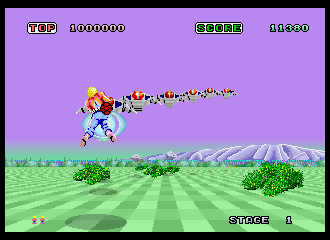
\includegraphics[width=.8\linewidth]{spaceharrier}
  \caption{\textit{Space Harrier} (1985)}
  \label{fig:sfig1}
\end{subfigure}
\begin{subfigure}{.5\textwidth}
  \centering
  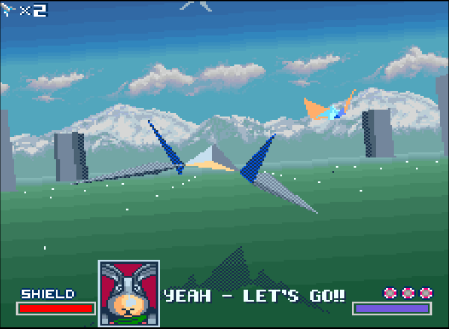
\includegraphics[width=.8\linewidth]{star_fox}
  \caption{\textit{Star Fox} (1993)}
  \label{fig:sfig2}
\end{subfigure}
\begin{subfigure}{.5\textwidth}
  \centering
  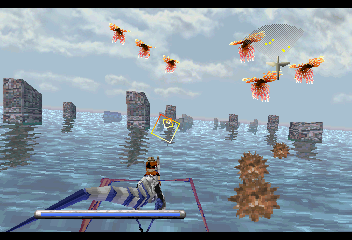
\includegraphics[width=.8\linewidth]{panzerdragoon}
  \caption{\textit{Panzer Dragoon} (1995)}
  \label{fig:sfig3}
\end{subfigure}
\begin{subfigure}{.5\textwidth}
  \centering
  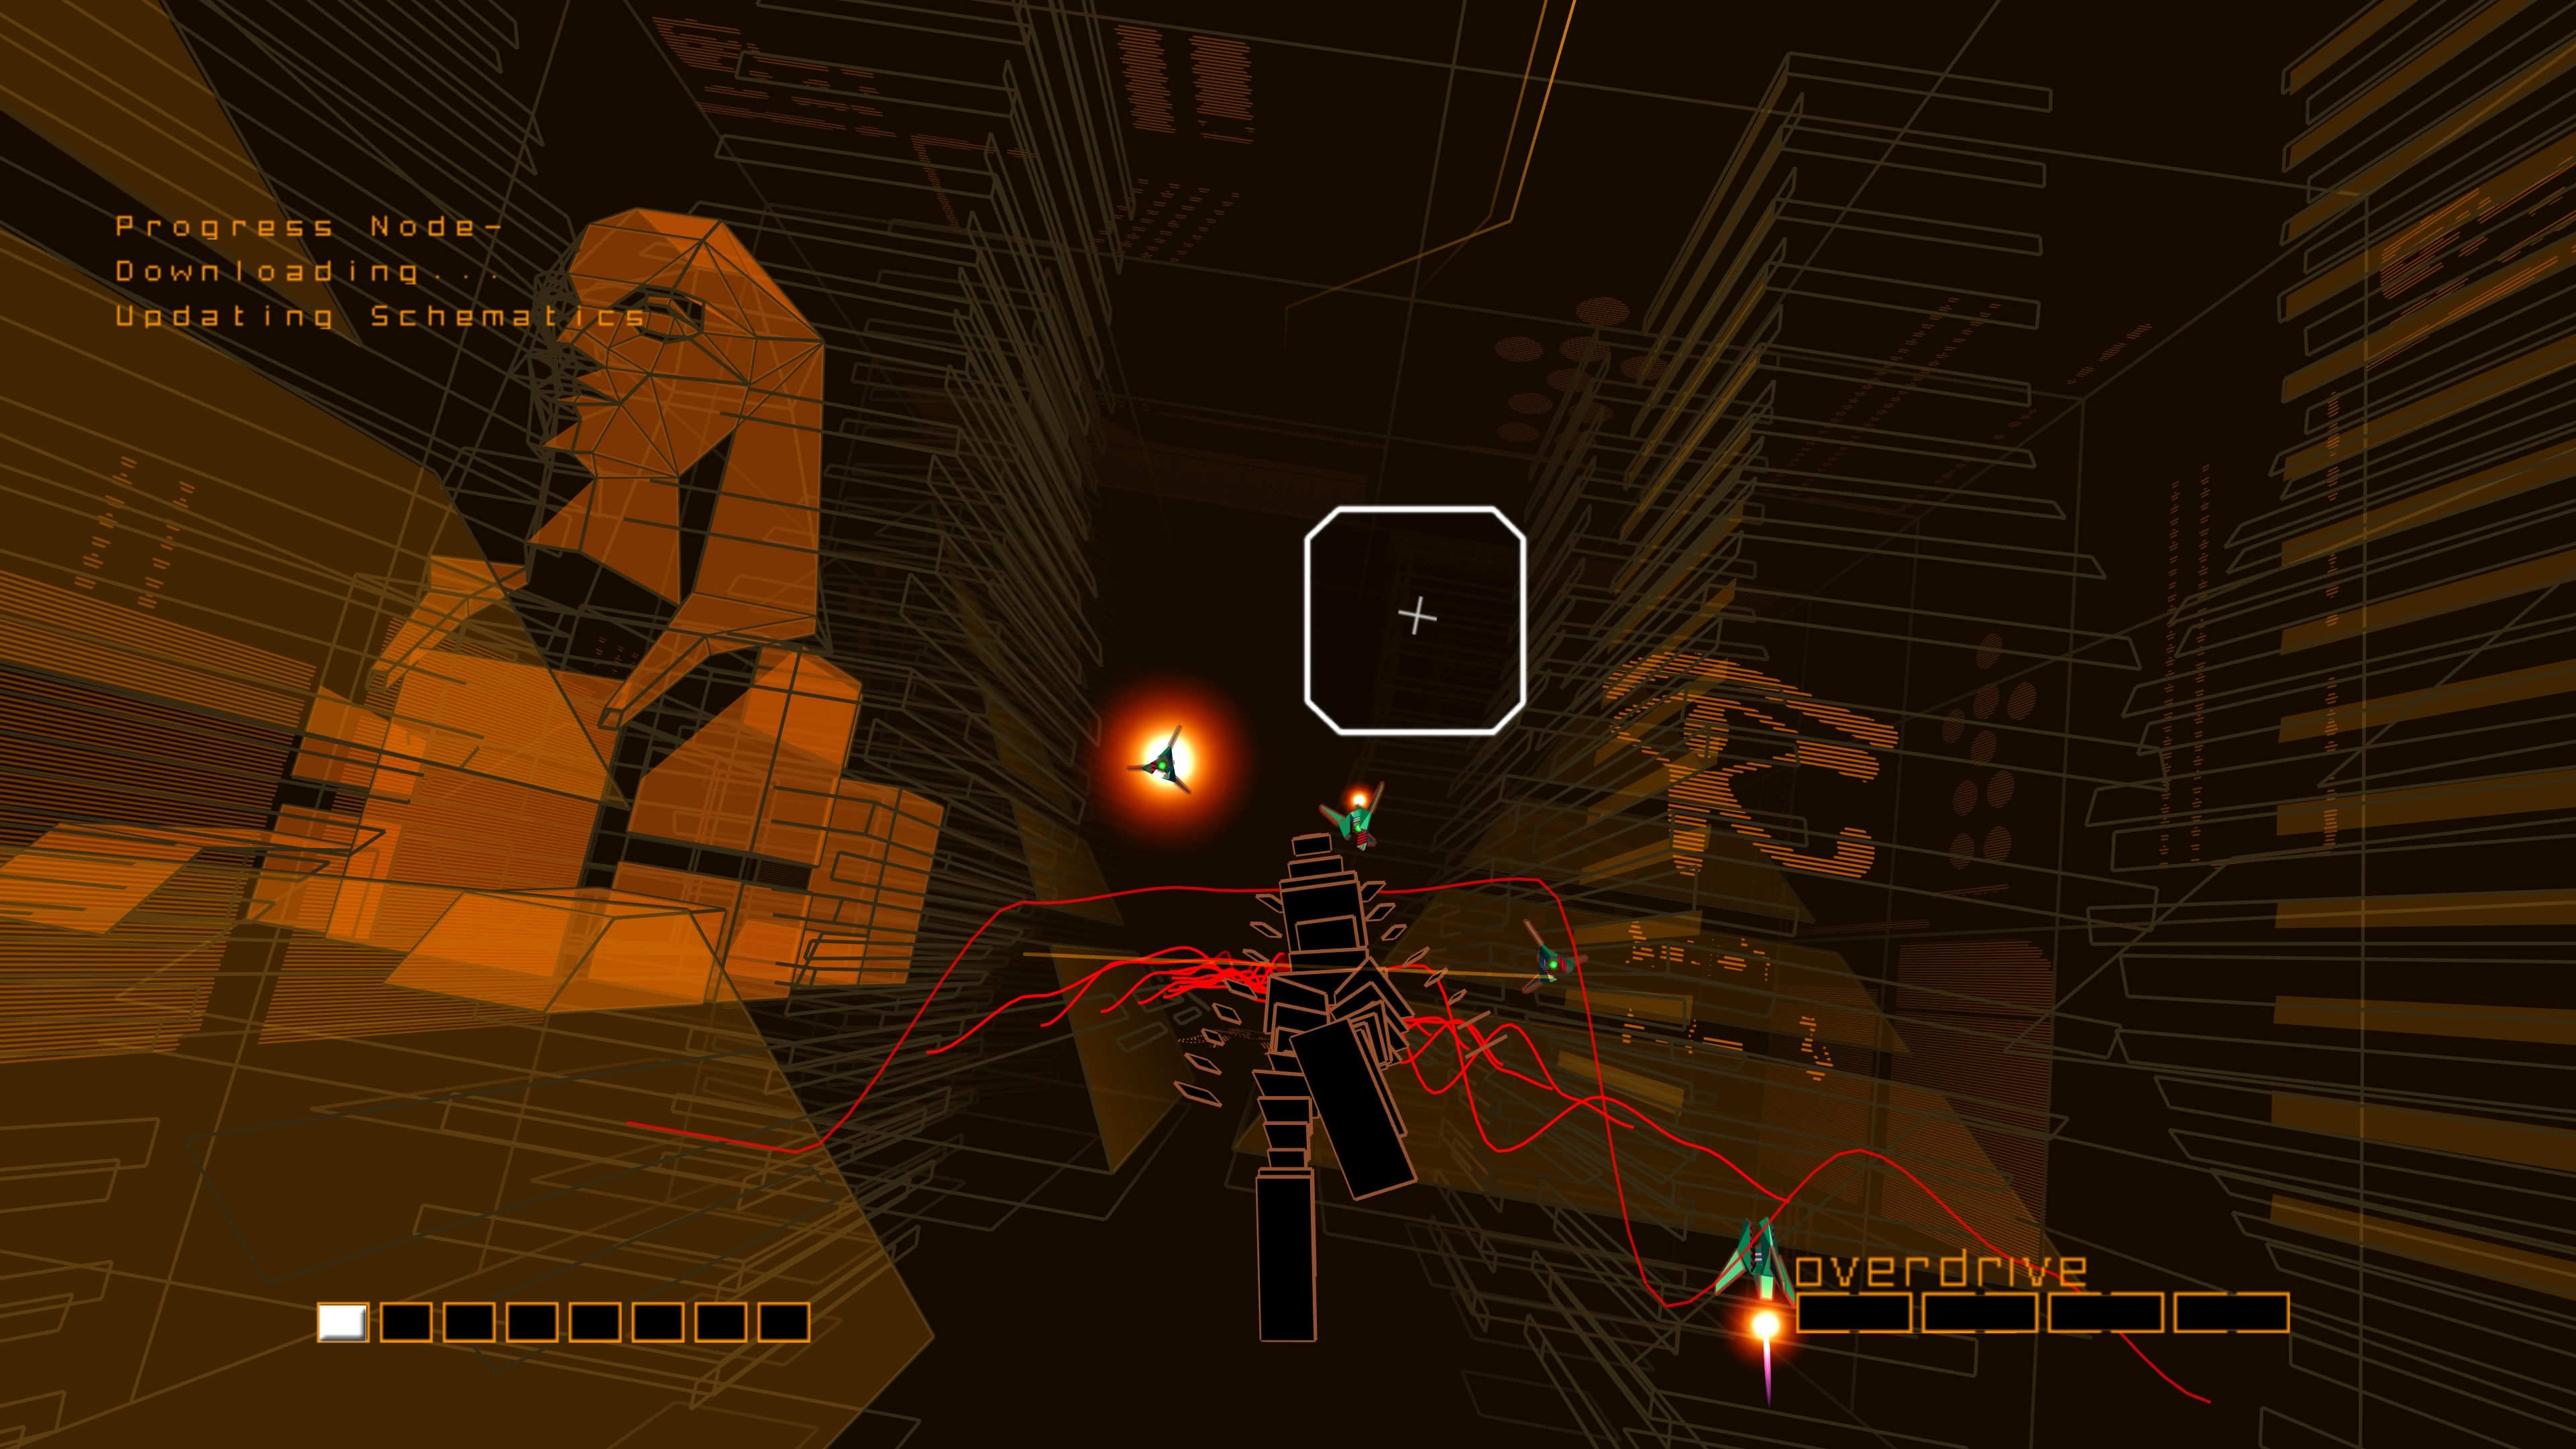
\includegraphics[width=.8\linewidth]{rez}
  \caption{\textit{Rez Infinite} (2016)}
  \label{fig:sfig4}
\end{subfigure}
\caption{four exemplar rail shooters}
\label{fig:history}
\end{figure}

\subsubsection*{Gameplay taxonomy}
% Describe the basic structure of a 3D rail shooter with reference to the above examples,
% outlining their various approaches to core gameplay elements like enemy design, player
% movement, shooting and targeting, significant action set-pieces, and their use of
% fixed perspective or a malleable 3D camera.

Rail shooters have a relatively straightforward gameplay structure, in which players are
automatically carried forward along a fixed path - within which they exercise a fairly
limited range of motion along their relative x-axis and y-axis, and within which they
shoot enemies, and avoid both environmental obstacles and incoming enemy fire. In early instances,
the player moves in a straight line with limited freedom to veer (without gameplay consequence),
while later entries in the genre guided players through more complex spatial compositions incorporating
curves and varied levels of elevation.

These games stand in contrast to games in two other related genres in ways which are illustrative.
They differ from gallery shooting games such as \textit{Virtua Cop} and \textit{House of the Dead}, which
often functioned with a physical gun peripheral, because the player remains in constant motion in
a rail shooter whereas gallery shooting games are generally played from a fixed position in the world
with player movement control typically limited to entering or exiting a form of cover and moving
between scenes. They also differ from aerial combat games such as \textit{Ace Combat} for the opposite
reason - whereas such games allow players to navigate their ship freely in 3D space, the rail shooter
confines movement to a fixed plane moving through a scripted path. As such, it may be fruitful to
define rail shooters, at the outset, as a genre of game concerned primarily with moving shooting galleries -
sitting in a distinct position between static shooting gallery games and freeform action combat games.

In these games, player movement typically doubles up as player aiming - in early iterations of the genre like
\textit{Space Harrier} and \textit{Star Fox}, movement is tied directly to the player's aim in a
linear fashion, and in later polygonal titles the player directly controls the player's targeting
reticle with player model movement following in an indirect fashion. This differs from modern 3D
game input systems in which player movement and player aiming are controlled independently via dual 
analogue control - this sequence of games were largely developed in tandem with the rise of 3D console
gaming, and largely fell out of fashion before dual analogue input became ubiquitous following the
2000 launch of Sony's PlayStation 2. \textit{Rez}, which launched following the launch of the PS2,
was still constrained by the Sega Dreamcast's single analogue input scheme.

% investigate camera controls in PD Orta, PD Remake, and Rez Infinite...

Although the games did not typical feature free camera control to aim in a dual analogue manner,
later games in the cycle did contain rudimentary camera controls. \textit{Panzer Dragoon}, for example,
allowed players to rotate the camera in 90 degree increments using the Sega Saturn's shoulder inputs.
Players were able to see the location of off-camera enemies via a radar in the heads up
display, requiring strategic decision making about which of four directions to shoot from.

This degree of freedom did not follow in all subsequent entries in the genre, highlighting the importance
of scripting from a design standpoint - in \textit{Rez} for example, camera rotations around the player
do occur, but without intervention from the player and in order to facilitate scripted action
set pieces that occur from different directions.

One point of departure explored by later games in the genre was the introduction of a lock-on mechanic,
allowing players to pre-target a group of enemies and release multiple shots by releasing the fire button.
This stands in contrast to traditional free firing approaches taken in earlier games. In \textit{Rez},
free firing is removed from the game entirely in favour of lock-on firing that allows the game to
better synchronise firing events (and their resultant sound effects) with the game's electronic score.

\subsection{PICO-8}\label{pico}

% Brief discussion of decision-making process involved in choosing PICO-8 as tool, with focus on
% project scope, interest in technical implementation details, and 3D modelling demands of building
% such a game in an off-the-shelf 3D game engine ala Unreal or Unity.

One of the initial decisions taken in the project was to settle on an appropriate technology
for building the software. The reasons for choosing PICO-8, and a brief introduction to the
system, will occupy the rest of this section.

The most obvious alternative was to use a fully featured off-the-shelf game engine such as
Unity or Godot. This was rejected at the outset for three principle reasons: firstly, the
use of an existing 3D engine with comprehensive given systems functionality (in, for example,
control and manipulation of 3D cameras and collision detection) would have shifted the focus
of the project away from systems implementation and towards less well defined design issues,
risking scope creep in a time-constrained project; secondly, the use of an existing 3D engine
would have increased expectations with regards to aesthetic fit and finish,
turning the project into an exercise in 3D modelling and texturing; and thirdly, these options 
would have introduced additional burdens in build and portability that are not shared by PICO-8.

The benefits of using off-the-shelf technology is discussed further, and retrospectively, in
Section \ref{engines}.

\subsubsection*{Introduction to PICO-8}
% Discuss ethos of PICO-8 as a ``fantasy console'' and outline its technical
% specification - emphasis on compute power, memory limitations, screen resolution,
% player inputs, and token limits - and indicate some of the implications of these
% constraints on project scope.

Developed by Joseph White, aka zep, and initially released in 2015, PICO-8 is a 
fantasy console modelled on the aesthetic of an 8-bit home console (such as,
for reference, the Nintendo Entertainement System or the Sega Master System).

The system is built around the following key constraints\cite{white}, which replicate
the aesthetic constraints of an 8-bit game console:

\begin{itemize}
   \item a 128x128 pixel display
   \item a fixed palette of 16 colours
   \item execution of four million virtual instructions per second
   \item a sheet of 128 8x8 sprites
\end{itemize}

% insert table of comparison - PICO vs NES vs MS vs SNES vs MD

Rough comparison of PICO-8 with popular home consoles of the 8-bit era, as
shown in Figure \ref{fig:consolecomparison}, reveals a system with roughly the same
compute power as the Master System and more than twice the compute of the Nintendo
Entertainment System (NES), while having a coarser pixel grid than either and
a more limited colour palette. Note that the emulated 4 MHz CPU of the PICO-8 system
is emulated by allowing four million virtual instructions per second and does not
map neatly to the actual performance of a hardware CPU clocked at 4 Mhz, where efficient
cycle utilisation is not guaranteed as it is in an emulated environment.

\begin{figure}[h]
\begin{center}
\begin{tabular}{r|c|c|c}
      & PICO-8 & Master System\cite{mastersystem} & NES\cite{nes} \\
     \hline
     CPU & 4 Mhz & 4 Mhz & 1.66 Mhz (PAL) \\
     Display & 128 x 128 & 256 x 192 & 256 x 240 \\
     Colour palette & 16 & 64 & 52 \\
\end{tabular}
\end{center}
\caption{PICO-8 compared to 8-bit home consoles}
\label{fig:consolecomparison}
\end{figure}

PICO-8 games are written in the a cut down version of the Lua scripting language -
schewing Lua's standard library and instead implementing a bespoke collection of
global functions. This is an advantage for PICO-8 as a tool for rapid prototyping and
experimentation, since Lua is a relatively light language that is easy to pick up and
use, and the choice of a simpler language also eliminates the overhead of complex
programming paradigms used in more typically used games programming languages such as
modern C++.

One oddity of the Lua programming language, particularly from the point of view of
game development, is that it is not a traditional object-oriented programming language
insofar as it does not have classes. Nonetheless, a form of prototype-based object orientation
is possible in the language and is used in the project. As the language's creator Roberto Ierusalimschy
explains\cite[p. 151]{ierusalimschy}, \say{each object may have a prototype, which is a regular object
where the first object looks up any operation that it does not know about. To represent a class in such
languages, we simply create an object to be used exclusively as a prototype for other objects
(its instances). Both classes and prototypes work as a place to put behavior to be shared by several
objects.}

Although we are using a prototype-based language that does not use classes, we will sometimes
use the expression 'class' to describe object prototypes for both convenience and familiarity.

\subsubsection*{PICO-8 as prototyping tool}
% Discuss benefits of using PICO-8 as a tool for rapid creation and iteration of
% game prototypes, compare and contrast to full 3D engines like Unity, Godot and Unreal,
% describe suitability given fixed time constraints of an individual summer
% project, and point to games successfully prototyped in PICO-8 (most notably
% \textit{Celeste}).

PICO-8 has significant advantages as a tool for rapid prototyping, and has been used
effectively as a prototyping tool for commercial game projects - most notably
acclaimed 2018 platformer \textit{Celeste}, which began life in a 2015 PICO-8 game jam.

The principle reasons for its effectiveness as a prototyping tool largely complement the
reasons for not adopting an off-the-shelf game engine, outlined above. Namely: PICO-8
has no complex build process and allows rapid tweaking and iteration; PICO-8 is extremely
portable and, because of its low demand on hardware, performance is guaranteed across a large
range of devices - allowing development to proceed with respect for a known and unchanging
frame budget; and the constraints generated by the system generally prevent scope creep and force
developer focus on essentials.

Additionally, while offering a lightweight development environment without the burdens
imposed by an off-the-shelf engine, PICO-8 does offer a fairly comprehensive suite of
features for getting game projects started quickly - including an \textunderscore update()
and \textunderscore draw()
loop to execute the game, facilities for drawing primitive objects and sprites
to the screen painlessly, simple controls for playing audio across four channels, and
in-built functionality for designing sprites and composing sound effects as shown in Figure
\ref{fig:pico}.

\begin{figure}[h]
\begin{subfigure}{.5\textwidth}
  \centering
  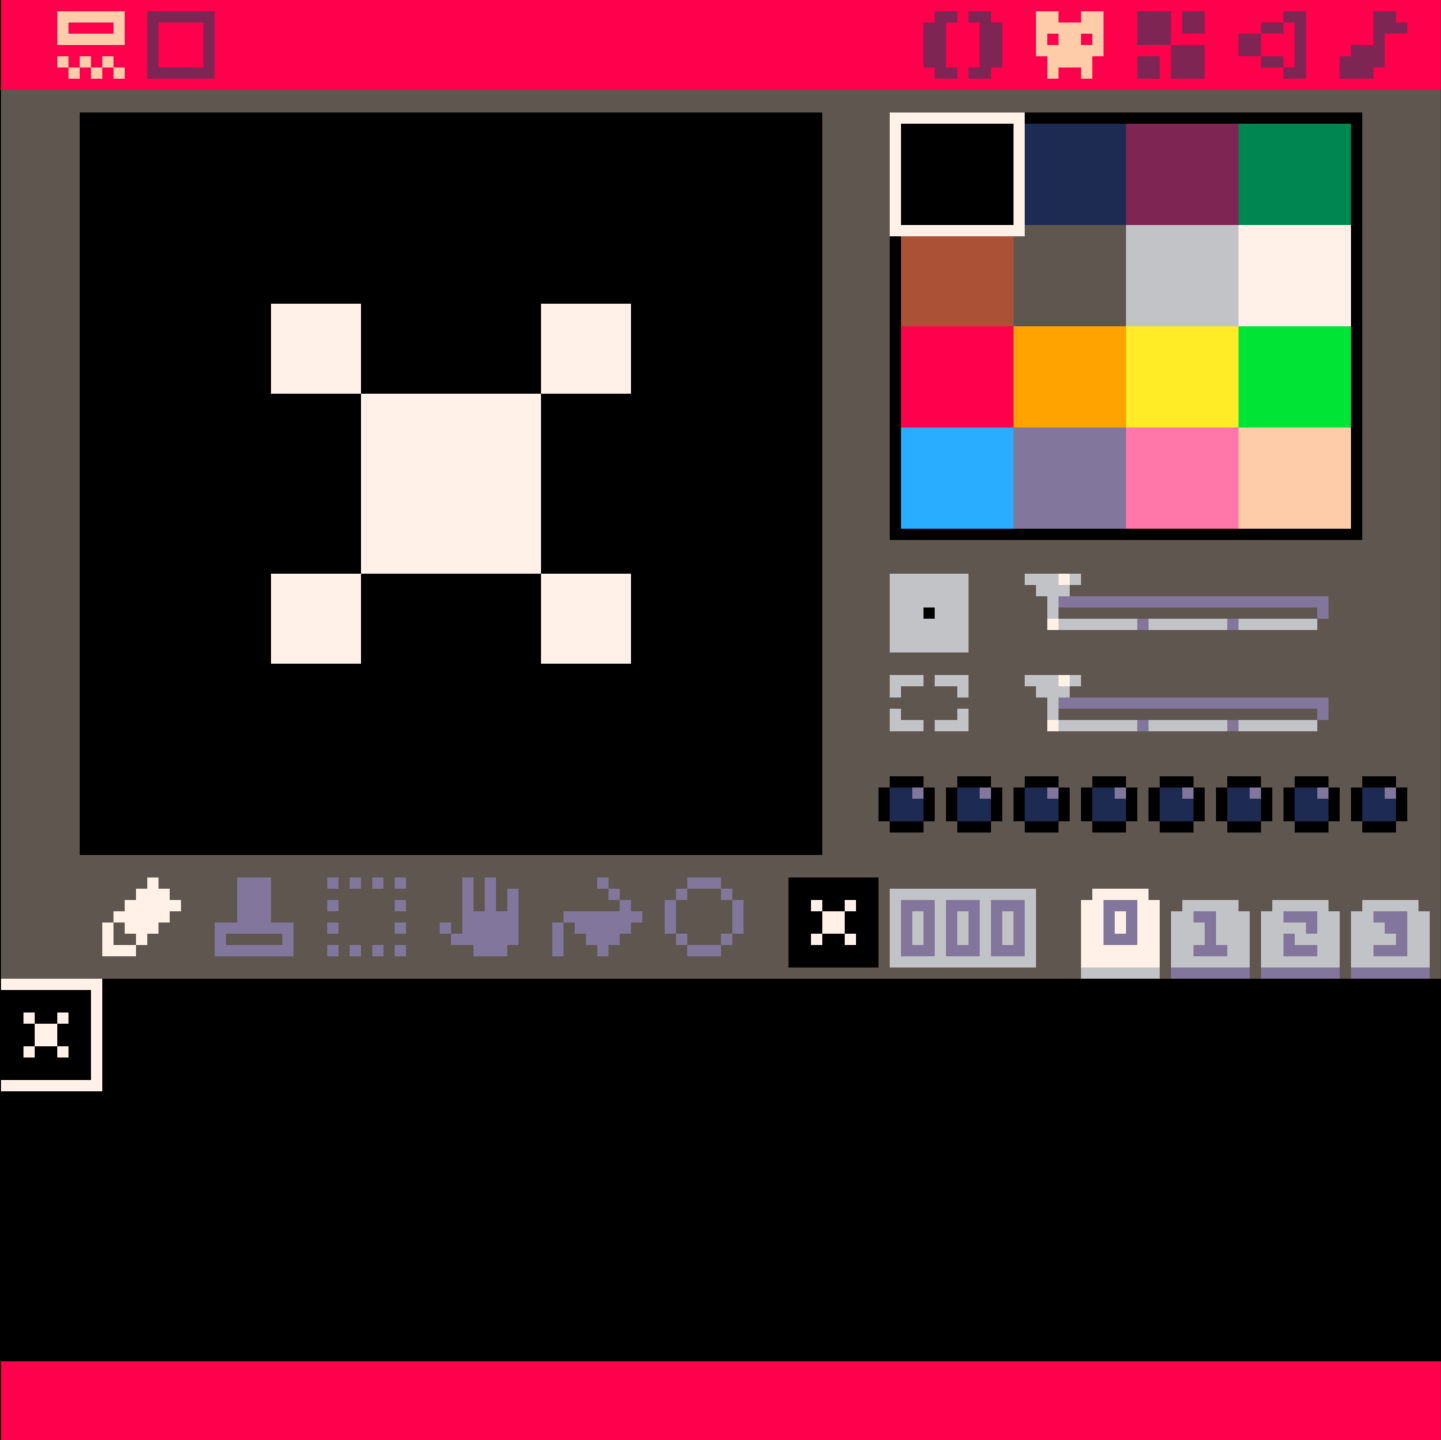
\includegraphics[width=.8\linewidth]{sprite_editor}
  \caption{PICO-8's in-built sprite editor}
  \label{fig:pfig1}
\end{subfigure}
\begin{subfigure}{.5\textwidth}
  \centering
  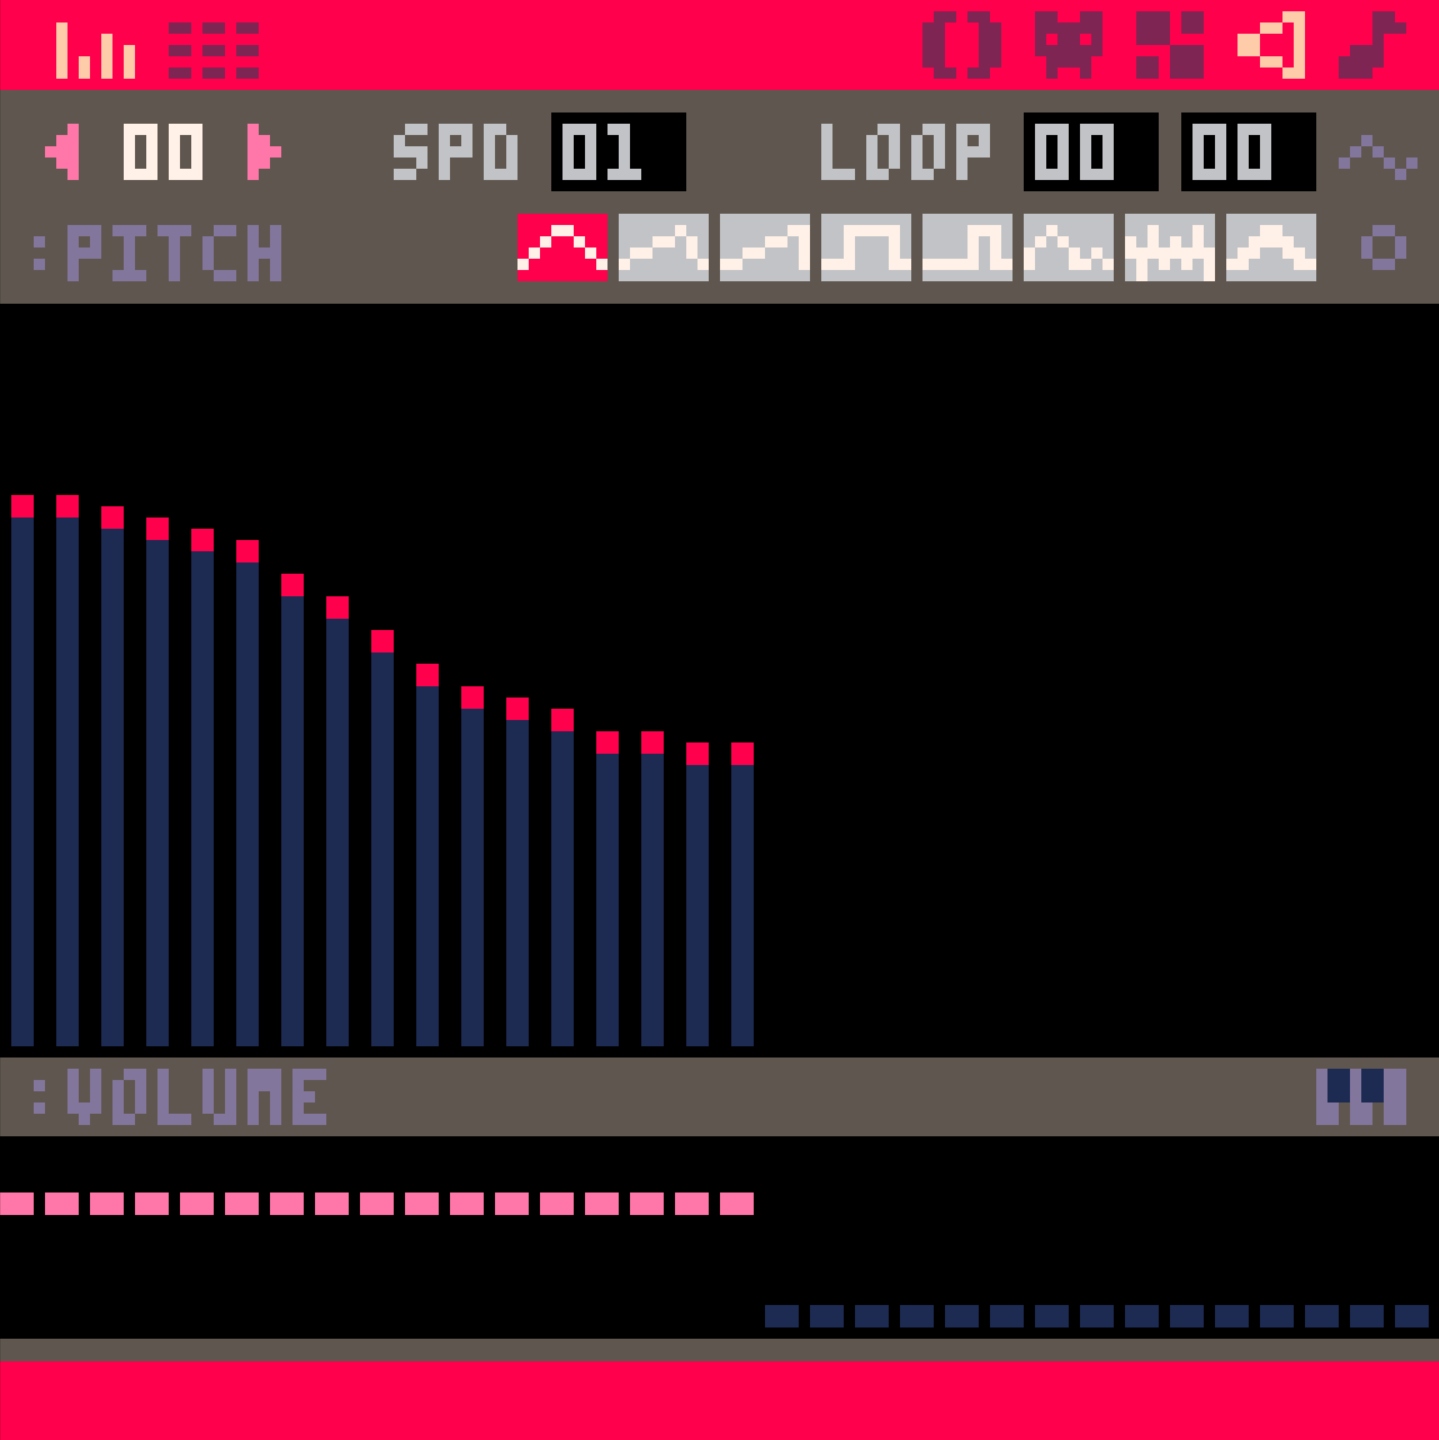
\includegraphics[width=.8\linewidth]{audio_editor}
  \caption{PICO-8's in-built audio editor}
  \label{fig:pfig2}
\end{subfigure}
\caption{PICO-8 asset creation suite}
\label{fig:pico}
\end{figure}

\subsubsection*{Sprite-scaling functionality}
% Discuss PICO-8's given functionality for sprite drawing and scaling and explain how
% these would facilitate development of a low-fidelity game utilising a pseudo-3D
% Super Scaler approach.
One specific advantage of using PICO-8 for this project, in addition to its general
advantages as a prototyping tool, is in-built support not only for drawing sprites
from a sheet but also for dynamically scaling sprites - the core rendering technique
that underlies the early Super Scaler games outlined in Section \ref{genre}.

In addition to the standard sprite drawing call spr() - which is ideally suited to
typical 2D games in which sprites are drawn at a constant size - PICO-8 also offers
an sspr() function that allows the programmer to dynamically scale and stretch sprites
by selecting the extreme corners of a rectangle in screen space into which the sprite
will be deformed and drawn. This, wrapped in functionality to project points in 3D space
to points on a 2D screen, allows the sort of sprite scaling that can simulate depth in 3D
space among multiple 2D sprite assets. This process is described in greater detail in
Section \ref{conversion}.

Where PICO-8 is disadvantaged is in the lack of support for arbitrary rotation of sprites -
a limitation imposed both by PICO-8's effort to emulate 8-bit games systems, which did not yet
have this facility, but also by the coarseness of the platform's pixel grid and the low fidelity
of accompanying sprites which resist easy and legible rotation around small angles. So, whereas late
Super Scaler games like \textit{After Burner} could increase immersion by easily allowing
camera tilting - simulating a degree of aircraft roll in that case - this project will
draw from a more limited set of possibilities in camera control.

\subsubsection*{Extensibility of 2D primitives for 3D}
% Discuss \textit{Star Fox} as exemplar polygonal rail shooter built within similar
% constraints and make critical comparison between PICO-8 platform specification and
% the Super Nintendo with on-cartridge Super FX graphics chip.
One ambition of this project, however, is to go a step beyond sprite scaling effects
and also introduce a limited degree of polygonal rendering - following the example of
Argonaut Software's 1993 Super Nintendo title \textit{Star Fox}, which leveraged bespoke
hardware to drive polygon rendering which is beyond PICO-8 only in scale.

% Discuss extensibility of PICO-8's functions for drawing primitives (eg rectfill and line)
% for triangle rasterisation and polygonal rendering.
Since, at root, polygonal rendering only requires the ability to draw triangles onto a
screen, PICO-8 can therefore perform the requisite functions if given primitive shape calls such
as line() and rectfill() are appropriately extended to draw filled shapes between three points.
The extension of these functions, to draw triangles and render polygonal models composed of
triangles, is discussed in Section \ref{prototyping}.

\subsubsection*{Mitigation strategies for constraints}
Given the known constraints of our chosen technology, it is worth considering in detail
the implications of some of these constraints and our proposed plans to mitigate against them
where possible.

% OOP

One of the most pressing constraints when developing for PICO-8 is the per-cart token
limit, which constrains the amount of code that can define your game. It is therefore
imperitive to practice good discipline in coding, avoiding code duplication and making use
of well structured object-oriented software architecture. PICO-8 carts are written in the
Lua scripting language, which is not traditionally object-oriented but which does have the
facilities to allow a form of prototype-based object orientation using metatables, as
discussed above. Therefore inheritance will be used to share core functionality across
like objects, preserving tokens to describe bespoke behaviours instead of code
duplication.
% use quotes from the Lua book 

% frame target ?? to keep or to cull...

Another obvious mitigation is to use the console's default 30Hz refresh mode rather than
the optional 60Hz mode. While faster refresh creates a more fluid and responsive game,
it trivially halves the frame budget, and the use of a 60Hz mode in such a constrained
environment, with ambitions to incorporate polygonal rendering, would introduce the
unnecessary risk of a significant bottleneck.

% blended approach

While the project aims to incorporate polygonal rendering, one important mitigation against
PICO-8's constraints is to not dogmatically adopt a purely polygonal approach and instead
opt for a blended approach that uses both polygonal and sprite-based rendering in a
blended way, allowing for more action on screen while allowing perspective-correct 3D models
in situations where they benefit the game. This blended approach, in which most objects are
rendered as sprites, also mitigates against another significant constraint of PICO-8: its
coarse pixel grid, which makes it hard to render polygonal shapes at small sizes legibly.

% multi cart

One further possible mitigation involves eschewing one of the system's constraints entirely.
PICO-8 does allow carts to load and run other carts, allowing developers to sidestep token
limits and build out multi-cart games, in which sections of the game are broken out into
separate discrete carts - perhaps sharing some assets and functionality - and then chained
together using load and run calls.

This approach will be discussed in more detail in Section \ref{multicart}, since it was an
approach ultimately taken in the final stretch of the project.

% Constraints

The choice of technology does also impose constraints that cannot be easily mitigated, and
instead will simply determine aspects of the game's design. As mentioned above, the system
does not have native support for sprite rotation and as such credible camera tilting is simply
not feasible as a technique.

Likewise, the limited number of player inputs (four directions and
two face buttons) minimise the range of actions available to the player - combinations of inputs
(for example, holding B while using directions) would allow us to expand the actions available
to the player, but at an obvious cost to intuition. This constraint can also be seen to
compound with other constraints - for example, a combination of face button and direction
button could facilitate real-time camera rotation, but the coarseness of PICO-8's pixel
grid would make it difficult to communicate the clear radar information required to
make decisions about camera control meaningful in the first place.

\section{Implementation I: Prototyping}

\subsection{Paper prototyping, software prototyping, and 3D rendering test}\label{prototyping}
The prototyping phase of the project began with three pieces of work along two tracks: firstly,
a paper prototype concretising the core gameplay loop, in which the player moves forward through
space and encounters enemies, and a software implementation of that paper prototype in PICO-8; and
secondly, initial technical work confirming the potential of PICO-8 for polygonal rendering and
introducing the basic ideas behind real-time polygonal rendering in general.

\subsubsection*{Basic player actions using primitives}

\begin{figure}[h]
\begin{subfigure}{.5\textwidth}
  \centering
  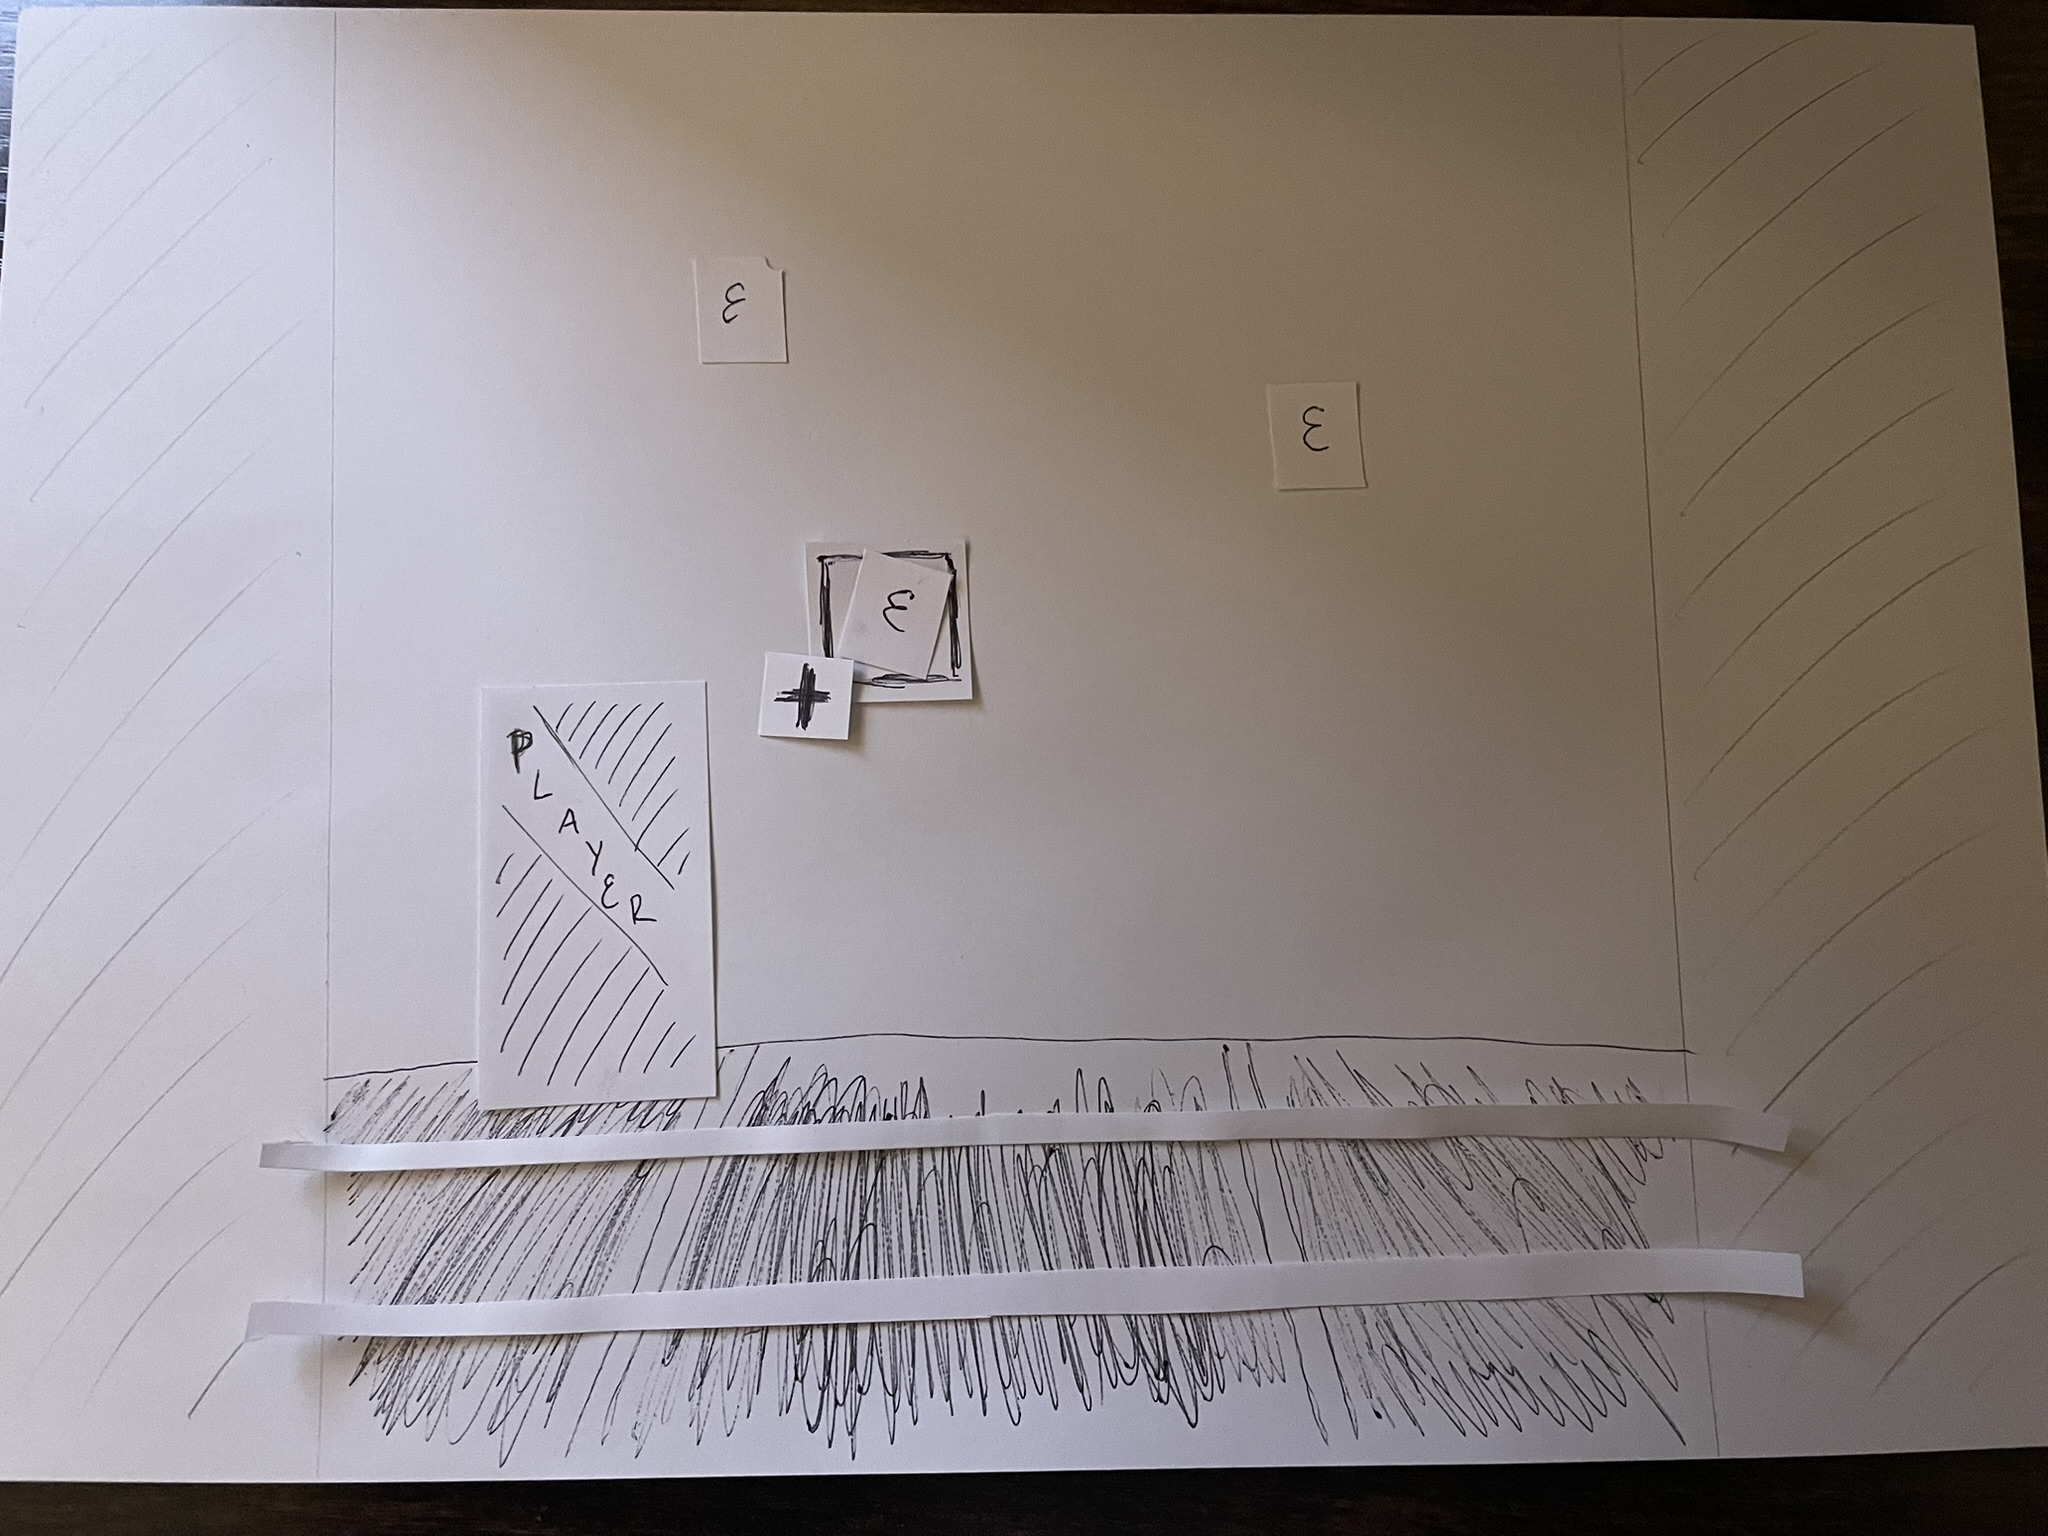
\includegraphics[width=.8\linewidth]{paper_prototype}
  \caption{paper prototype}
  \label{fig:pfig1}
\end{subfigure}
\begin{subfigure}{.5\textwidth}
  \centering
  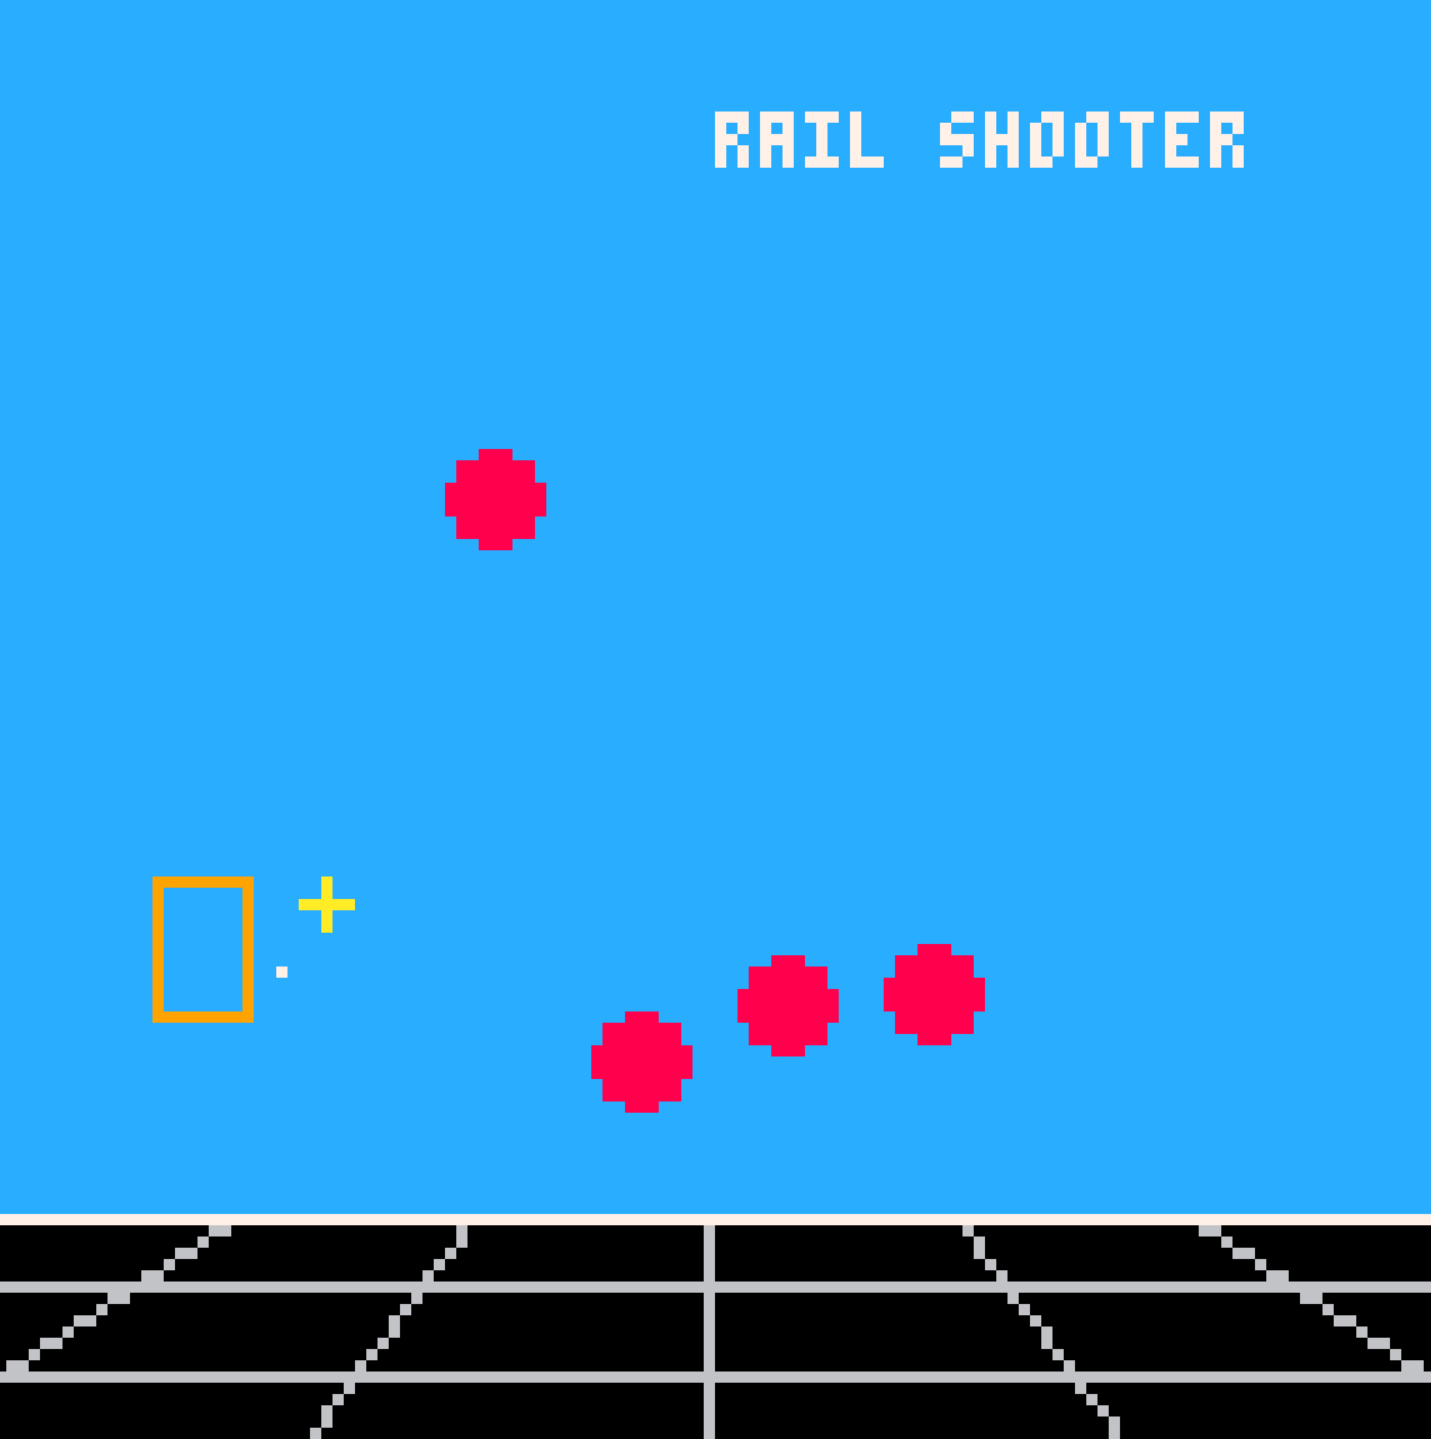
\includegraphics[width=.8\linewidth]{prototype2d}
  \caption{initial software prototype}
  \label{fig:pfig2}
\end{subfigure}
\caption{early prototyping}
\label{fig:gameprototype}
\end{figure}

% Referring back to the gameplay taxonomy conducted in the background section, explain
% how the most significant user actions were distilled down to fit a six-input
% gamepad. Showcase how this was modelled using a flat paper prototype and outline
% how this was translated into a software prototype using primitive shapes to model
% the player and randomly spawned enemies, with movement and interactions being
% directly translated into screen-space.

The primary purpose of the initial paper prototype was to distill the core essence of the
genre, as outlined in the gameplay taxonomy of Section \ref{genre}, into an interactive
medium that allowed easy play with various gameplay elements - examining, for example,
the possible relationships between a player sprite and its firing reticle, and possible
patterns of enemy movement.

Because of the limitations of prototyping on paper, this
phase focused on fairly linear gameplay in which the player moved forward along a straight
path and encountered enemies who existed along a single hypothetical plane in front of
the player, as can be seen in \ref{fig:pfig1}.

Several basic features of the game were explored through this prototype, including the
motion of projectiles in screen space between the player sprite and its reticle, the
motion of enemy projectiles towards the player, and the use of a lock-on mechanic akin to
that implemented in \textit{Panzer Dragoon} and \textit{Rez}.

Elements were also constructed to experiment with the naive simulation of a scrolling
floor - using fixed white perspective lines on a filled rectangle supplemented by
scrolling horizontal lines replicating the phenomenon of forward movement.

Following construction of this rudimentary paper prototype, work began on a light software
prototype describing the same basic game behaviours, as seen in \ref{fig:pfig2}, based on the
use of PICO-8's drawing functions for primitive shapes - in this case, rect(), rectfill(),
circfill(), and line().

In this version, the player primarily controls the firing reticle rather than the player sprite,
with the relationship between sprite and reticle defined by their distance from the centre of the
screen - the player reticle is bound to an internal box in screen space, and to create an easy
illusion of depth, the player sprite (here simply a hollow rectangle) is drawn closer to the
real edge of the screen by a linear factor.

Developing out of the paper prototype, much of the logic of this initial software prototype occurs
in screen space, rather than being projected out from a hypothecated 3D world space. Advancing on
the paper prototype, a simple illusion of movement in depth is given to the circular enemy shapes
through naive enlargement in screen space, but bullets still move linearly across the screen instead
of accurately rendering perspective-correct movement through depth.

% Highlight issues already identified at this early stage of prototyping - such as
% player model blocking, the relationship between the player reticle and the destination
% of projectiles in hypothecated 3D space, the need for limitations on enemy
% target locking, and the need for game objects to have a meaningful existence in 3D
% space.

The benefits and pitfalls of paper prototyping for a 3D game project, and its impact on the
direction of the initial software prototype, are discussed further and retrospectively in
Section \ref{prototypepitfalls}.

Ultimately, in addition to developing comfort with the basic structure of the game and beginning
to define its basic behaviours, the paper prototype and initial software prototype revealed the
need to start grappling with the design of a correct 3D system, in which objects have positions
in depth as well as along the axes of a screen. This phase of development will be discussed in
Section \ref{conversion}.

\subsubsection*{Simple 3D renderer with model scaling and rotations}\label{renderer}

% Describe the contruction of a simple 3D renderer to prove suitability of PICO-8 for
% the proposed project. Expose and discuss my implementation of triangle rasterisation
% in PICO-8 and briefly explain the benefits of decomposing 3D shapes into triangles
% rather than quads. Discuss related issues in polygonal rendering such as triangle
% sorting and backface culling.

While working on the initial software prototype outlined above, a second course of work
was followed to confirm the capacity of PICO-8 to render polygonal models and to begin
building the required functionality over and above PICO-8's primitive drawing functions.

Firstly, a simple algorithm was implemented to draw a filled triangle between three points
in screen space, using line-by-line rect() calls to draw lines between appropriate points on the
sides of the triangle. The rectangular draw function rect() is used
rather than the more intuitive line() function, because PICO-8's implementation of line drawing
includes additional overhead to calculate best fitting lines between diagonal points, even when
drawing lines between two points that share a position on one axis.

Triangles are used as the building block for polygonal rendering because three points, which define
a plane in 3D space, guarantee stable flat surfaces - whereas quad rendering can produce surfaces
between points that are under-described, with a fourth point sitting on a different plane to the
other three and creating ambiguities in the relation of points across a surface. It should be
noted, however, that nothing forces us to use triangles - and indeed the Sega Saturn did render
polygonal graphics using texture mapped quads.

% triangle algorithm

In order to render triangles, the coordinate points of the three corners of the triangle are first sorted by their
\textit{y}-axis position so that we can draw them consistently from top to bottom. The per-line step required to
draw the long side is then calculated by dividing the \textit{x}-axis distance between the highest and lowest point
by their distance in \textit{y}.

The two shorter sides are then calculated by performing the same operation between the highest
and middle points, and again between the middle point and the lowest point. Appropriate logic is
included to handle edge cases too - for example, where two or three points share a position in
\textit{y}.

The triangle can then be filled using these three increments on a line-by-line basis - moving down
the pixel grid one line at a time and drawing 1 pixel width rectangles between \textit{x}-axis coordinates
defined by the position of the top corner of the triangle, and incremented in both directions by the per-line
step derived above. This is done in two phases - from the top corner to the middle corner, using the per-line
steps found for the long edge and the top-most short edge, and then from the middle corner to the bottom
corner using the per-line steps for the long edge and the bottom-most short edge.

% point projection

Once triangle drawing functionality was built, functionality to translate 3D coordinates onto
screen space was required. This was done through the use of point projection calculations which
will be discussed in more detail in Section \ref{conversion},
where its broader application to the game software itself will be covered.

% description of 3D models

But we still need to describe the triangle, in world space, that we are projecting onto a camera in the
first place. 3D models are described by giving the position of their vertices in 3D model space - that is,
with the object centred around origin (0, 0, 0). The vertices are then connected
in data defining the triangles they form in the model, with points listed in clockwise order from
the outside to establish their orientation and enable efficiency techniques like backface culling
(a process, not applicable to all circumstances as we will see in Section \ref{boss}, by which we
do not draw faces that do not face us).

We can then apply a range of transformations to the vertices thus defined, easily scaling
the model around origin (0, 0, 0) by direct multiplication of coordinates, and rotating
objects using well defined and readily available rotation matrices.

Once scale and rotation operations have been applied in model space, the object can then be
placed in world space simply by translating each of its vertices by the object's position vector.

Once the core rendering functionality had been built for a single cube, the functionality
was subjected to a simple ``sanity test'' to establish confidence that the performance
cost of polygonal rendering in PICO-8 was not too heavy to preclude its use in the
game.

Using common model space data, nine cubes were defined in our PICO-8 cart with simple inputs
to cycle through the numbers being rendered at any one time and to freely rotate all cubes.
Figure \ref{fig:3dprototype} outlines the results of the testing with backface culling enabled, showing
significant headroom for game logic even with nine cubes rendered at once.

\begin{figure}[h]
  \centering
  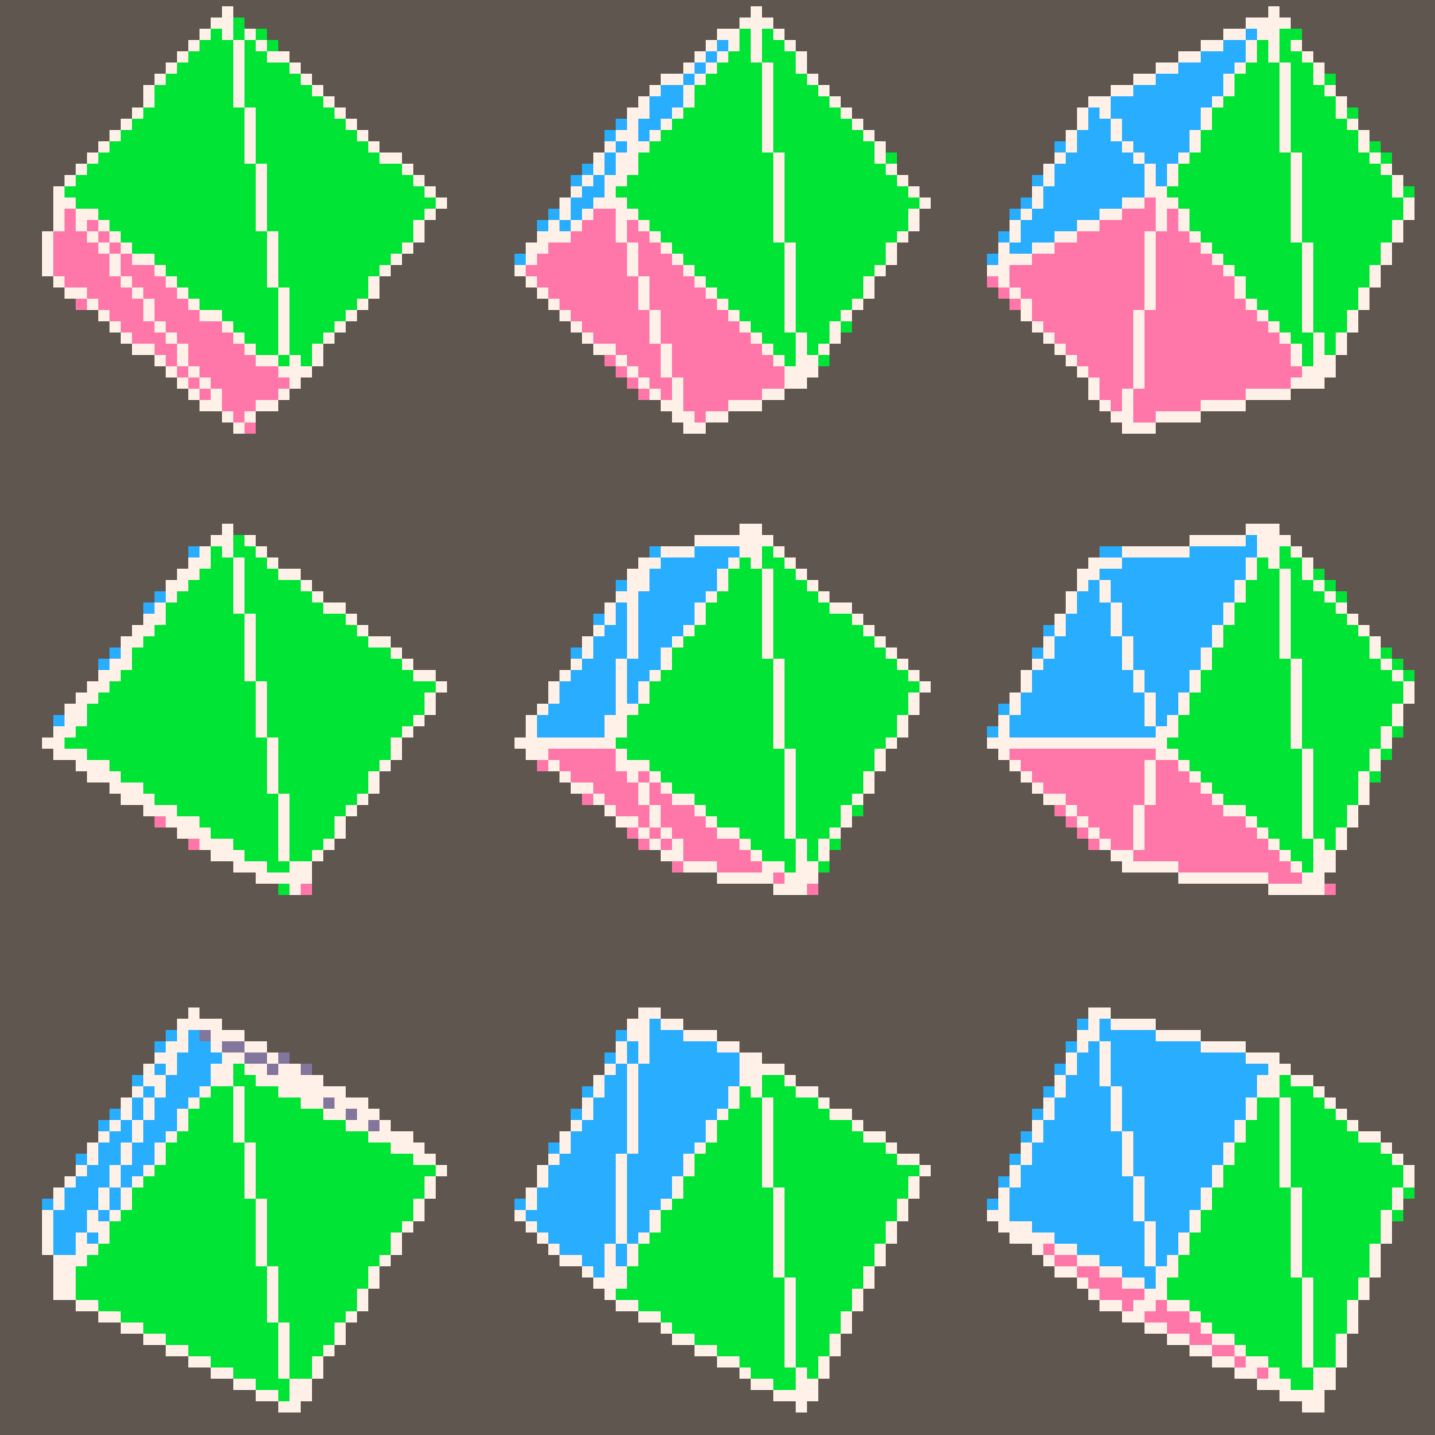
\includegraphics[width=.8\linewidth]{test3d}
  \caption{multi-cube sanity check}
  \label{fig:3dfig2}
\end{figure}

\begin{figure}[h]
\begin{center}
\begin{tabular}{r|c c c c c c c c c c}
     Cubes drawn & 0 & 1 & 2 & 3 & 4 & 5 & 6 & 7 & 8 & 9 \\
     \hline
     CPU utilisation & .37 & .39 & .41 & .43 & .46 & .47 & .49 & .50 & .52 & .53
\end{tabular}
\end{center}
\caption{CPU load sanity testing results}
\label{fig:3dtest}
\end{figure}

\subsection{3D conversion of software prototype}\label{conversion}

While the initial software prototype served a useful purpose in creating familiarity
with the basic mechanics and feel of the game, and sparking early thinking about some of the
significant design decisions that needed to be made, its origins in a flat paper prototype
also led to key technical implementation issues being elided - namely the accurate handling
of depth and perspective necessary to properly deliver on the initial idea of the project.

As such, the initial software prototype was built on in the next phase of development and refactored
so that objects carried proper three-dimensional positions in world space, and were drawn in a
properly scaled and perspective correct way instead of having movement in depth faked through
arbitrary re-scaling in screen space. Likewise, collision handling was re-written to accurately detect
intersections of bounding volumes in three-dimensional space, instead of being handled through
screen space intersection in a 2D plane.

Note at the outset: for the purposes of this project we are using a left-handed Cartsean coordinate
system to describe both world space and model space, in which the positive \textit{x}-axis faces right,
the positive \textit{y}-axis faces up, and the positive \textit{z}-axis faces forward.

\subsubsection*{Perspective-correct 3D projection and scaling}
% Discuss the application of 3D point projection to the corners of 2D sprite objects
% to achieve perspective correct drawing and scaling of 2D elements using PICO-8's sspr
% function. Highlight use of small camera movements (spatial displacement in x and y)
% aligned to player sprite movement to heighten illusion of depth along the z-axis.
One of the key changes introduced in this 3D software prototype was the creation of accurate
depth among enemy units, created by correctly projecting sprite objects onto the screen using
newly introduced \textit{z}-coordinate values.

In order to accurately project a point from 3D space onto a screen, we must hypothecate a viewport in 3D space
and a camera position, and then exploit the law of similar triangles to identify the point in space at
which the line between the point and our camera - which will be positioned at the origin of the
coordinate system, (0, 0, 0), for simplicity - intersects with our viewport.

\begin{figure}
   \centering
   \begin{tikzpicture}
      [scale = 1.5,
      axis/.style={-stealth},
      dot/.style= {
         draw,
         fill = black,
         circle,
         inner sep = 0pt,
         minimum size = 4pt
      },
      point/.style= {
         draw,
         fill = black,
         circle,
         inner sep = 0pt,
         minimum size = 2pt
      }]
      
      \draw[axis] (-0.5, 0) -- (5, 0) node[right] {$z$};
      \draw[axis] (0, -0.5) -- (0, 2) node[above] {$y$};
      \draw (1, -0.25) -- (1, 1.5) node[above] {$V$};

      \draw (3, 1.5) node[dot, label = {right:$P$}] {};
      \draw (3, 1.5) -- (3, 0);
      \draw (3, 1.5) -- (0, 0);

      \draw (0, 0) node[below left] {$O$};
      \draw (1, 0) node[below left] {$A$};
      \draw (3, 0) node[below] {$B$};
      \draw (1, 0.5) node[dot, label = {above left:$P'$}] {};

   \end{tikzpicture}
   \caption{side orthographic view of a point projection on the \textit{y}-axis, adapted from figure 9-2 of Gambetta
   \cite[p. 106]{gambetta}}
   \label{fig:triangles}
\end{figure}

This operation must be performed along both the $x$ and $y$ axes, and figure \ref{fig:triangles}
illustrates how the law of similar triangles can be used to determine viewport projection of point $P$
in the $y$-axis as an example, giving us the point $P'$ that describes the $y$-coordinate of
the point's projection on our viewport\cite[p. 106]{gambetta}.

Because triangles $OBP$ and $OAP'$ are similar triangles - that is, they are right angled triangles that have the same
internal angles - we can leverage the fact that, as similar triangles, the ratio of their equivalent sides is the same.

Therefore we can say that the ratio of lengths $OA$ and $AP'$ is the same as the ratio of lengths $OB$ and $BP$. If we know
the coordinate position of point $P$, and know that our camera is situated at origin $O$, we know that the length of $OB$ is
simply the $z$-coordinate of the point $P$ and $BP$ is its position in $y$. We also know that length $OA$ is simply the
distance between the camera and the viewport - a distance which we know because we have hypothecated these objects in
3D space ourselves. As a consequence, the length of the line $AP'$ is:

\begin{equation}
   |AP'| = \frac{|BP| * |OA|} {|OB|}
\end{equation}

or, the $y$ coordinate of the point, projected onto the viewport $V$, is:

\begin{equation}
   V_y = \frac{P_y * V_z} {P_z}
\end{equation}

Once this calculation is made, we simply need to translate the figures for our actual screen or canvas, which uses different
measures from our in-scene viewport, and this is achieved by multiplying the calculated coordinate by the width ($C_w$) or height 
($C_h$) of our canvas in pixels (128 in both axes in PICO-8), and dividing this by the in-scene width ($V_w$) or height ($V_h$) of
our viewport. To take as an example the calculation of the $y$-coordinate position of our point on the screen:

\begin{equation}
   C_y = \frac{\frac{P_y * V_z} {P_z} * C_h} {V_h}
\end{equation}

This calculation can be simplified by hypothecating a 1 by 1 in-scene viewport and
a viewport distance of 1 in $z$ - since any number divided or multiplied by 1 remains unchanged, we can simply eliminate
arbitrary multiplications and divisions from our computation and scale our scenes for this set-up. The downside of this approach,
however, is that it does lock us into a particular field of view. The simplified equation is as follows, again for the $y$ coordinate
calculation:

\begin{equation}
   C_y = \frac{P_y} {P_z} * C_h
\end{equation}

Finally, the position value must be adjusted to account for the fact that the centre of our in-scene viewport looks directly
along the \textit{z}-axis along \textit{x}, \textit{y} coordinates of (0, 0), whereas (0, 0) on our canvas exists
in the top left corner of the screen rather than the centre, and the positive direction of \textit{y} is therefore
inverted on our screen too.

This entire operation is implemented in the code highlighted in figure \ref{fig:codeproject} using a single short function
that takes a three-component vector - representing the \textit{x}, \textit{y}, and \textit{z} coordinates of a
vertex in space - and projects them onto a viewport of width and height 1, centred around (0, 0) and located
one unit along the \textit{z}-axis. This returns two values, for screen projection in \textit{x} and \textit{y}.

\begin{figure}[h]
   \begin{lstlisting}
project_vert = function(vect3)

   return 64 + (((vect3[1] - camera.x) / vect3[3]) * 128),
           64 - (((vect3[2] - camera.y) / vect3[3]) * 128)

end
   \end{lstlisting}
   \caption{vertex projection function}
   \label{fig:codeproject}
\end{figure}

This function is called twice for each sprite drawn, finding the position of the top-left and bottom-right
corners of its face - derived from an object's position, its width, and its height - and then drawing the
sprite using PICO-8's in-built scaled sprite function sspr(), discussed in Section \ref{pico}.

Figure \ref{fig:projection} illustrates how this process renders scenes using perspective projection.
While it highlights the use of this function to project the extreme corners of 2D sprites onto a screen,
the same method is also used by the program to project the three vertices of triangles onto screen space
too - allowing the rendering of polygonal shapes such as the player ship and the icosahedral boss enemy shell,
or the polygonal cubes discussed in the previous section. Discussion of \textit{z}-sorting to ensure proper
ordering as well as proper scaling of objects will be picked up in Section \ref{draw}.

\begin{figure}[h]
\begin{subfigure}{.3\textwidth}
   \centering
   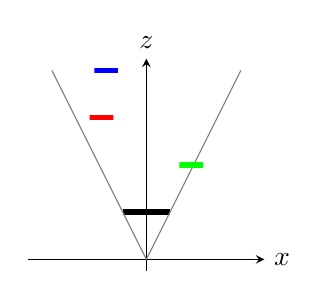
\begin{tikzpicture}
      [scale = .6,
      axis/.style={-stealth},
      dot/.style= {
         draw,
         fill = black,
         circle,
         inner sep = 0pt,
         minimum size = 4pt
      },
      point/.style= {
         draw,
         fill = black,
         circle,
         inner sep = 0pt,
         minimum size = 2pt
      }]
      
      \draw[axis] (-2.5, 0) -- (2.5, 0) node[right] {$x$};
      \draw[axis] (0, -0.25) -- (0, 4.25) node[above] {$z$};

      \draw[line width = 2] (-0.5, 1) -- (0.5, 1);
      \draw[draw = gray] (0, 0) -- (-2, 4);
      \draw[draw = gray] (0, 0) -- (2, 4);

      \draw[line width = 2, draw = blue] (-1.1, 4) rectangle (-0.6, 4);
      \draw[line width = 2, draw = red] (-1.2, 3) rectangle (-0.7, 3);
      \draw[line width = 2, draw = green] (0.7, 2) rectangle (1.2, 2);

   \end{tikzpicture}
   \caption{top orthographic view of a game scene}
   \label{fig:rotfig1}
\end{subfigure}\hfill
\begin{subfigure}{.3\textwidth}
   \centering
   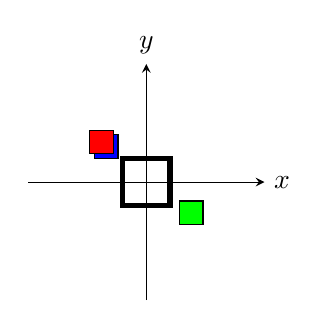
\begin{tikzpicture}
      [scale = .6,
      axis/.style={-stealth},
      dot/.style= {
         draw,
         fill = black,
         circle,
         inner sep = 0pt,
         minimum size = 4pt
      },
      point/.style= {
         draw,
         fill = black,
         circle,
         inner sep = 0pt,
         minimum size = 2pt
      }]
      
      \draw[axis] (-2.5, 0) -- (2.5, 0) node[right] {$x$};
      \draw[axis] (0, -2.5) -- (0, 2.5) node[above] {$y$};

      \draw[fill = blue] (-1.1, 1) rectangle (-0.6, 0.5);
      \draw[fill = red] (-1.2, 1.1) rectangle (-0.7, 0.6);
      \draw[fill = green] (0.7, -0.4) rectangle (1.2, -0.9);
      \draw[line width = 2] (-0.5, -0.5) rectangle (0.5, 0.5);

   \end{tikzpicture}
   \caption{front orthographic view of a game scene}
   \label{fig:rotfig1}
\end{subfigure}\hfill
\begin{subfigure}{.3\textwidth}
   \centering
   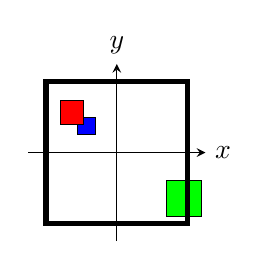
\begin{tikzpicture}
      [scale = 1.8,
      axis/.style={-stealth},
      dot/.style= {
         draw,
         fill = black,
         circle,
         inner sep = 0pt,
         minimum size = 4pt
      },
      point/.style= {
         draw,
         fill = black,
         circle,
         inner sep = 0pt,
         minimum size = 2pt
      }]
      \draw[axis] (-0.625, 0) -- (0.625, 0) node[right] {$x$};
      \draw[axis] (0, -0.625) -- (0, 0.625) node[above] {$y$};

      \draw[fill = blue] (-0.275, 0.25) rectangle (-0.15, 0.125);
      \draw[fill = red] (-0.4, 0.367) rectangle (-0.233, 0.2);
      \draw[fill = green] (0.35, -0.2) rectangle (0.6, -0.45);

      \draw[line width = 2] (0.5, 0.5) rectangle (-0.5, -0.5);


   \end{tikzpicture}
   \caption{perspective-correct projection of sprite objects onto screen}
   \label{fig:rotfig2}
\end{subfigure}\hfill
\caption{projection of a sprite objects in 3D space onto a canvas}
\label{fig:projection}
\end{figure}

\subsubsection*{Real-time 3D collisions}

% Discuss implementation of cuboid bounding volumes to test for collisions, using
% height, width, and depth data paired if three-dimensional positions to check for
% intersection of volumes. Discuss the need for axis-alignment to significantly
% simplify calculations, and the design implications of this with regard to rotational
% symmetry of objects depicted (ie disc-shaped saucers, and spherical projectiles)

Having translated the game into 3D world space for the purposes of perspective-correct rendering, adjusting
the game's collision system was the next logical step.

In the initial software prototype, without \textit{z} values to work with, single pixel projectiles were simply
fired across the screen in a 2D plane with simple checks to see if they had entered the player (represented in
the initial prototype as a hollow rectangle) or enemies (represented as solid circles). This became untenable
as a solution, given that it jarred with perspective-correct rendering of enemy units, and the prototype was
updated to test for collisions using cuboid bounding volumes.

Cuboid bounding volumes can have two principal uses in a collision detection system. In complex simulations,
checks for intersection between cuboid volumes can be used as a pruning mechanism - an initial approximation
to either disconfirm that intersection has occurred, or else call for a more complex test of the actual
geometry being bounded. In more simple systems, such as the low-fidelity game being built in this project,
cuboid volumes can be used effectively to test for collisions in general\cite[p. 75]{ericson}.

Two of the most desirable characteristics of bounding volumes are tightness of fit with underlying geometry,
and ease of rotation and transformation\cite[p. 76]{ericson}. As such, an early design decision was made to
populate the game with objects that are exactly (or close to exactly) rotationally symmetrical.

Therefore projectiles are depicted as spheres, rather than taking on a tapered bullet-shaped appearance. The main
enemy units are depicted as round flying saucers. Both objects can be represented in collision space in
axis-aligned cuboid bounding volumes that do not need to rotate at all to reflect any putative rotation of
the object in space, significantly simplifying intersection calculations.

Although these bounding volumes are not perfect matches for the objects being represented, they are sufficiently
tightly bound to simulate a plausible system of collisions - to quote Christer Ericson, veteran programmer of Sony
Santa Monica and NeverSoft, ``in games, collision detection and response can effectively be governed by `if it looks
right, it is right.' Other applications have stricter accuracy requirements\cite[p. 12]{ericson}.''

\begin{figure}[h]
\centering
\begin{subfigure}{.45\textwidth}
   \centering
   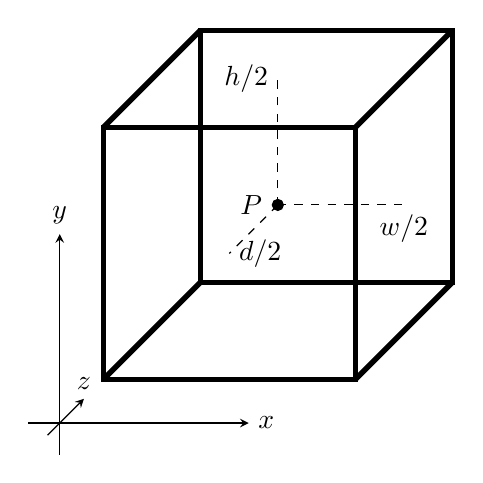
\begin{tikzpicture}
      [scale = 0.8,
      axis/.style={-stealth},
      dot/.style= {
         draw,
         fill = black,
         circle,
         inner sep = 0pt,
         minimum size = 4pt
      },
      point/.style= {
         draw,
         fill = black,
         circle,
         inner sep = 0pt,
         minimum size = 2pt
      }]
      
      \draw[axis] (-0.5, 0, 0) -- (3, 0, 0) node[right] {$x$};
      \draw[axis] (0, -0.5, 0) -- (0, 3, 0) node[above] {$y$};
      \draw[axis] (0, 0, 0.5) -- (0, 0, -1) node[above] {$z$};

      \draw[line width = 2] (0.5, 4.5, -0.5) rectangle (4.5, 0.5, -0.5);
      \draw[line width = 2] (0.5, 4.5, -4.5) rectangle (4.5, 0.5, -4.5);
      \draw[line width = 2] (0.5, 4.5, -0.5) -- (0.5, 4.5, -4.5);
      \draw[line width = 2] (0.5, 0.5, -0.5) -- (0.5, 0.5, -4.5);
      \draw[line width = 2] (4.5, 4.5, -0.5) -- (4.5, 4.5, -4.5);
      \draw[line width = 2] (4.5, 0.5, -0.5) -- (4.5, 0.5, -4.5);

      \draw (2.5, 2.5, -2.5) node[dot, label = {left:$P$}] {};
      \draw [dashed] (2.5, 2.5, -2.5) -- (4.5, 2.5, -2.5) node[below] {$w/2$};
      \draw [dashed] (2.5, 2.5, -2.5) -- (2.5, 4.5, -2.5) node[left] {$h/2$};
      \draw [dashed] (2.5, 2.5, -2.5) -- (2.5, 2.5, -0.5) node[right] {$d/2$};

   \end{tikzpicture}
   \caption{a centre-radius bounding representation defined by position \textit{P}, height \textit{h},
   width \textit{w}, and depth \textit{d}}
   \label{fig:colfig1}
\end{subfigure}\hfill
\begin{subfigure}{.45\textwidth}
   \centering
   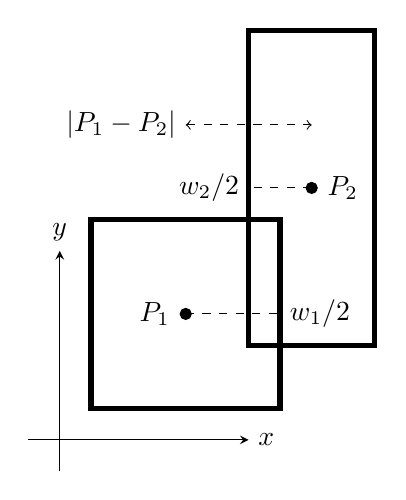
\begin{tikzpicture}
      [scale = 0.8,
      axis/.style={-stealth},
      dot/.style= {
         draw,
         fill = black,
         circle,
         inner sep = 0pt,
         minimum size = 4pt
      },
      point/.style= {
         draw,
         fill = black,
         circle,
         inner sep = 0pt,
         minimum size = 2pt
      }]
      
      \draw[axis] (-0.5, 0) -- (3, 0) node[right] {$x$};
      \draw[axis] (0, -0.5) -- (0, 3) node[above] {$y$};

      \draw[line width = 2] (0.5, 0.5) rectangle (3.5, 3.5);
      \draw (2, 2) node[dot, label = {left:$P_1$}] {};
      \draw[line width = 2] (3, 1.5) rectangle (5, 6.5);
      \draw (4, 4) node[dot, label = {right:$P_2$}] {};

      \draw [dashed] (2, 2) -- (3.5, 2) node[right] {$w_1/2$};
      \draw [dashed] (4, 4) -- (3, 4) node[left] {$w_2/2$};
      \draw [dashed, <->] (2, 5) node[left] {$|P_1-P_2|$} -- (4, 5);

   \end{tikzpicture}
   \caption{front orthographic projection of an intersection check of two volumes, showing comparison along a single axis}
   \label{fig:colfig2}
\end{subfigure}\hfill
\caption{collision of axis-aligned cuboid bounding volumes}
\label{fig:collision}
\end{figure}

Since the game records the position of game objects through a single three-coordinate vector at the object's
centre, axis-aligned bounding volumes use a centre-radius representation\cite[p. 78]{ericson}, as seen in
figure \ref{fig:colfig1}, in which the bounds of the volume are defined by positional data and values for the
object's height, width, and depth - of which height and width are already used for rendering.

Collisions between objects of this representation are then calculated using a simple series of checks comparing
the distance between the objects on each axis by the difference of their radius along that axis as
depicted in figure \ref{fig:colfig2} - here derived as the sum of their relevant extensions divided by two such
that we can say collision occurs when:

\begin{equation}
   |P_1 - P_2| < \frac{e_1 + e_2} {2}
\end{equation}

This is implemented in code in figure \ref{fig:codecollide}.

\begin{figure}[h]
   \begin{lstlisting}
collides = function(body1, body2)

   return abs(body1.x - body2.x) < (body1.width + body2.width)/2 and
         abs(body1.y - body2.y) < (body1.height + body2.height)/2 and
         abs(body1.z - body2.z) < (body1.depth + body2.depth)/2

end
   \end{lstlisting}
   \caption{a boolean check for collision between two axis-aligned bounding volumes}
   \label{fig:codecollide}
\end{figure}

Several known optimisations have been eschewed in this implementation due to token limits in PICO-8
imposing a cost to additional code overhead, in addition to the fact that collision-related performance
bottlenecks have not been encountered - in no small part due to the design decisions mentioned above.

Therefore, for example, spatial partitioning has not been implemented. Under this scheme the quadratic time
complexity of checking for collision between all objects in the world is controlled via a divide-and-conquer
strategy that partitions the game world into disjoint sets, and only tests for collisions between objects that
reside in the same approximate area of the world.

But a more bespoke form of divide-and-conquer strategy has been implemented to reduce the number of pairwise collision
checks, and avoid the quadratic time complexity of naively testing all combinations, by only checking for collisions
between specific classes of object and rendering other collisions irrelevant to the game. As such, collision checking - 
as we will see in Section \ref{update} - is handled within the update() function of each object that may be subject to
a collision with significance for the game, instead of collisions being handled by a single global function.

For example, the player can collide with enemy projectiles and drone enemies, but no check is performed
for collisions with saucer enemies since their behaviour is such that they never share a horizontal
plane with the player. Likewise, saucer enemies do not check for collisions with other saucers - they are 
assumed not to collide, and when collisions do happen in the game world the graphical low-fidelity of the
game allows their intersection to be interpreted perceptually as close-by rather than intersecting motion -
and, as such, any such intersection has no consequence that needs to be resolved.

\subsubsection*{Graphical effects with 2D sprites and particles}

As indicated in the prior section, techniques to simplify the process of 3D collision detection naturally
suggested particular decisions for the graphical design of the game - namely a bias towards using rotationally
symmetrical objects that can be bound to axis-aligned cuboid bounding volumes without concern about object
rotation in world space.

As such, representations of enemy units as primitive circles were replaced with a simple sprite representing
a flying saucer as seen in Figure \ref{fig:saucer} - an easily identifiable object, consistent with a science-fiction theme,
that contains the rough rotational symmetry required by the simplified collision system.

Destruction effects were also added to the game, composed of two components - an animated explosion, which
served as the background to the effect, and a foreground system of particles in randomly assigned colours
drawn from the sprite of the destroyed object.

Explosions - represented like other projected objects through a 3D position vector and radius information -
are animated using progressive radius expansion at a semi-random rate assigned on object initialisation.
Further animation within the sprite was achieved inexpensively by leveraging the xflip and yflip parameters
of PICO-8's sspr() function, which allows sprites to be flipped independently in either, neither, or both of the
\textit{x} and \textit{y} axes. By adding a simple timer to the objects, we are able to create the illusion of
organic motion within the explosion sprite by arbitrary flipping over time - exploiting intentional asymmetries
in the sprite's pixel grid as seen in Figure \ref{fig:explosion_sprite}.

\begin{figure}[h]
\begin{subfigure}{.45\textwidth}
  \centering
  
\includegraphics[width=.8\linewidth]{ship_sprite}
  \caption{a sprite depicting a rotationally symmetrical flying saucer enemy, represented by a cuboid
  bounding box}
  \label{fig:saucer}
\end{subfigure}\hfill
\begin{subfigure}{.45\textwidth}
  \centering
  
\includegraphics[width=.8\linewidth]{explosion_sprite}
  \caption{an explosion sprite with intentional asymmetries, to simulate animation through sprite flipping}
  \label{fig:explosion_sprite}
\end{subfigure}\hfill
\caption{sprite designs}
\label{fig:sprites}
\end{figure}

Particles, likewise, are spawned on the destruction of an enemy in semi-random numbers and assigned semi-random
values to make the effect feel unscripted and organic. Particles are assigned colour values corresponding to
values found in the original enemy sprite, creating an illusion of debris, and then assigned random directions
and speed factors that execute over a given number of subsequent frames against the backdrop of a randomly
expanding and flipping explosion animation.

% Describe the implementation of 2D sprites to replace primitive shapes used in earlier
% iterations of the prototype. Discuss the design considerations that led to the
% adoption of easily identifiable flying saucer and drone designs. Discuss simple
% graphical effects used to eg light up flying saucer lights, or spin rotors of
% enemy drones. Explain implementation of enemy destruction effects - namely the
% implementation of a simple particle system over the bed of an explosion animation
% efficiently faked by a combination of progressive scaling and random flipping of a
% non-symmetrical sprite.

\section{Implementation II: Full implementation}

Following extensive prototyping and the development of a functional software version that
implemented the core intended gameplay loop and incorporated perspective-correct sprite projection,
polygonal rendering, and real-time collision detection in 3D space, it was time to start work on
the final implementation - starting with a properly designed software architecture and object
hierarchy that built on the lessons of early prototyping and properly ordered the software in
a rational, DRY, and polymorphic way.

In addition to a significant ground-up reworking of the second software prototype, development
also began on the end-game boss - featuring a more interactive polygonal element and associated
problems with 3D geometry. This phase of the project also, ultimately, saw the project shift toward
a multicart design following a late encounter with PICO-8 token limits.

\subsection{Settled software architecture and object hierarchy}
As discussed in Section \ref{pico}, Lua is not a traditionally object-oriented programming
languages with classes. As such, object orientation is achieved through object prototyping and
is here implemented at cart initialisation through the comprehensive setting of metatables
to define the intended hierarchy of classes (or, rather, object prototypes) as shown in Figure
\ref{fig:codeinheretance}.

\begin{figure}[h]
   \begin{lstlisting}
function _init()

   -- set up inheritance heirarchy
   setmetatable(sprite_object, {__index = game_object})
   setmetatable(polygonal_object, {__index = game_object})

   -- tables that inherit from sprite_object
   setmetatable(scenery_object, {__index = sprite_object})
   setmetatable(enemy, {__index = sprite_object})
   setmetatable(drone, {__index = sprite_object})
   setmetatable(explosion, {__index = sprite_object})
   setmetatable(pickup, {__index = sprite_object})
   setmetatable(bullet, {__index = sprite_object})

   -- tables that inherit from polygonal_object
   setmetatable(player, {__index = polygonal_object})

end
   \end{lstlisting}
   \caption{a prototype-based inheritance hierarchy established at cart initialisation}
   \label{fig:codeinheritance}
\end{figure}

As can be seen, the software is structured around a fairly simple and shallow inheritance hierarchy,
in which a base game\textunderscore object has two subclasses - sprite\textunderscore object and
polygonal\textunderscore object - from which most other renderable objects in the game inherit.
These two subclasses of the base class define the core drawing functionality of each kind of object.

The rest of the game is structured around composition, with a persistent game\textunderscore world object
containing a sequential series of wave objects, containing enemies and defining their behaviour as a group.
The operations of these objects will be discussed in detail in Section \ref{update}.

\subsection{The core game loop}
As discussed in Section \ref{pico}, PICO-8 gives the developer the basic functionality
of a game loop - namely, \textunderscore update() and \textunderscore draw() functions that
are called repeatedly to
simulate and render the action of the game at the chosen refresh rate (here, 30Hz).
In this section, we will walk through the logic implemented in each of these two functions
to execute the game - referring back to Section \ref{conversion} where appropriate, if
functionality was carried over from the earlier 3D prototype.

\begin{figure}[h]
    \centering
    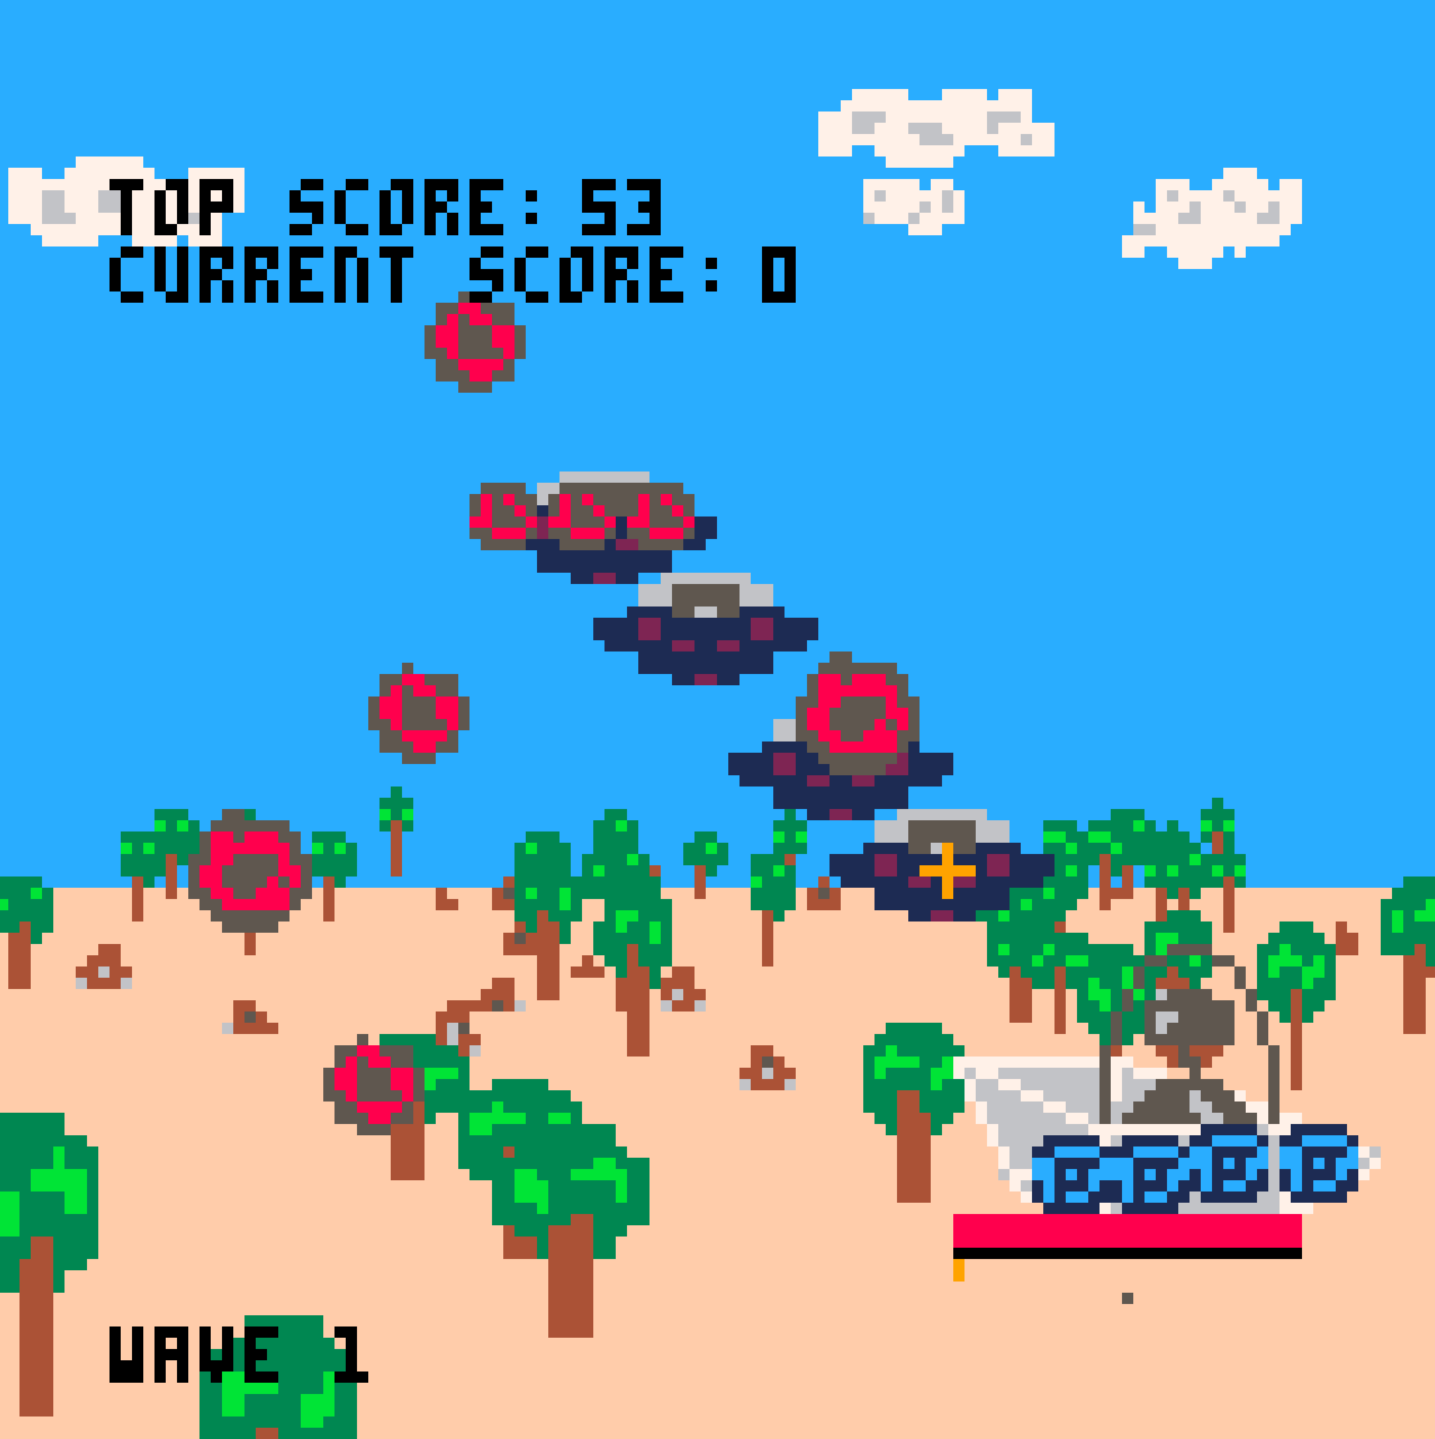
\includegraphics[width=.8\textwidth]{final3d}
    \caption{final software}
    \label{fig:3dfinal}
\end{figure}

\subsection{The update loop}\label{update}

\subsubsection*{Updating the gameworld}
The given \textunderscore update() loop present in the main game file simply calls one
function: the update() function of the game\textunderscore world object.

First we perform a simple check for player death with a branch that executes if the
life of our player is less than or equal to zero. If this is the case, we check if
the player's current score is higher than the cart's high score, and reassign the
cart's high score in persistent cart data if so. Finally, we pass control back to
a game\textunderscore over cart with a load() call, from which the player can restart the
main game cart.

If the player has not died, control passes to logic that controls our current enemy
wave. We will discuss the internal functioning of enemy waves below, but at a high level
we check if a wave has been completed and, if so, adjust the global
speed\textunderscore factor of the game as a naive tuner for escalating difficulty
(see below for more information on difficulty scaling).

If a wave has been completed and we have not reached our maximum number of pre-boss waves,
we initialise a new wave and increment our wave counter - as well as spawning one of three
potential in-game pick-ups to reward players between waves, offering replenished health,
additional lock-on capacity, or a reduced lock-on cooldown.

If we have reached the final wave, we instead call a function to store our existing scenery
in PICO-8 memory and make a load() call to run the cart containing our boss encounter (discussed
below in Section \ref{boss}).

After this logic has executed, and assuming we have not loaded the boss encounter
cart, the game will run the update function of its current wave - either deriving
the next frame's worth of activity for our current enemy wave, or else deriving the
first frame's worth of activity for our newly initialised wave.

We then update our player - taking and handling any user input, and testing for
appropriate collisions - before finally managing our scenery, fired projectiles,
and various spawned pick-ups, essentially incrementing their movement by one frame to
simulate scrolling (in the case of scenery and pick-ups) or projectile movement.

\subsubsection*{Speed scaling as a proxy for difficulty}

Before continuing to discuss the update() method of the wave object, we should briefly discuss the use of
a global speed\textunderscore factor variable to increment difficulty across a run of the game.

NASA-TLX perceived workload testing\cite{nasa} was performed on five subjects to identify the effectiveness of
tweaking two aspects of game speed on perceived workload, taken here as a proxy for difficulty. The test
was structured by asking players to complete a ten-wave run of the game on the default build of the game, on
a version that was tweaked to scale enemy movement speed more rapidly than enemy fire rate, and a version that
was tweaked to scale enemy fire rate more rapidly than enemy movement speed. The results are presented in tabular
form in Figure \ref{tlx}. The three tasks were given in a random order to each participant to mitigate learning
effects across the cohort.

\begin{figure}[h]
\begin{center}
\begin{tabular}{r|c|c|c}
      & Control build & Accelerated enemy speed & Accelerated enemy fire rate \\
     \hline
     P1 & 39 & 52 & 67 \\
     P2 & 67 & 88 & 64 \\
     P3 & 29 & 67 & 36 \\
     P4 & 69 & 84 & 74 \\
     P5 & 42 & 45 & 34 \\
     \hline
     Average & 49.2 & 67.2 & 55 \\
\end{tabular}
\end{center}
\caption{Raw TLX scores for perceived workload across three different game builds}
\label{fig:tlx}
\end{figure}

As expected, both forms of scaling presented greater perceived workload than the default build of
the game on average - although both Participant 2 and Participant 5 found the fire rate augmented
task less demanding than the default build of the game. No participant found less perceived
workload in the movement augmented build than in the default build.

Because both factors are shown to be, to some degree, effective levers of workload, the game
maintained a uniform speed\textunderscore factor variable that controlled both in a linear fashion,
although data showing that enemy movement carries greater weight in setting difficulty than enemy
fire rate could inform future work in creating more carefully calibrated user-selected difficulty
settings for the game.

\subsubsection*{Updating the current enemy wave}

The wave object's update() method can be broken down neatly into two sections: the first
of which executes the specific behaviour of this subclass of wave, and the second of
which executes generic updating tasks common to all types of enemy wave present in
the game.

At initialisation, a wave takes one one of four forms depending on the current
game\textunderscore world wave counter. These four forms describe enemy waves in which,
respectively, the incoming enemy ships are either saucers that move in a sweeping motion,
saucers that move in a circular motion, saucers that move in a spreading motion,
or are drone enemies who attack the player in a ``Kamikaze'' fashion.

Once initialised - ie, once the newly created object has been set to one of these
four modes, each with a unique internal update method - the wave, once updated by the
game\textunderscore world update() function, will call its own internal
class\textunderscore update() method in order to execute the behaviour of one of
the four subtypes. This largely consists of timer-based control over the spawn of
enemies up to a limit.

Once this class\textunderscore update() is complete, the wave table carries out
more generalised hygiene on the enemies it contains.

Firstly, the update() method iterates through the enemies it contains and
checks whether or not they were marked as destroyed during the previous frame.
If so, a new explosion is initiated at their current position and they are
subsequently removed from the list of enemies - along with a point of score being
awarded to the player and a simple explosion sound effect being called.

Then, enemies are tested for position - if they have moved behind the viewport,
they are considered off-screen and are removed from the wave's table of enemies.
Since we define the behaviour of enemies and have determined that they move
contrarywise to the player at all times, we can safely assume that they will
not return.

We then iterate through the wave's table of ongoing explosions, and remove those
that have expired (ie, their internal counter has reached zero).

Once that has been done, we update first all of our enemies and then all of
our explosions. The enemy update() function will be discussed below. The
explosion update() function is significantly simpler and broadly executes
the animation logic of progressive sprite expansion and quasi-random flipping
outlined in Section \ref{conversion}.

Once all enemies and explosions have been updated, we make a final check to
see if the wave has been completed - that is, that the wave has persisted for
more than 300 frames or ten seconds (the chosen time window across which a
wave will spawn its enemies) and there are no enemies or explosions remaining.
If so, the wave is marked as completed and the game\textunderscore world update()
function will initialise a new one in the next frame as discussed above.

\subsubsection*{Updating individual enemies}

The update() function of individual enemies can be broken down into four main steps: checking for
player target locking, checking for collisions with projectiles, updating its position to simulate
movement, and controlling its own firing routine.

Firstly, target locking is handled in the enemy object in the course of ordinary gameplay by comparing
the \textit{x} and \textit{y} positions of the enemy unit with the corresponding coordinates of the
player - in essence, checking if the player is looking at the object down the \textit{z}-axis. If so,
and if the player is holding fire (as ascertained through a flag that will be discussed below), we then
handle logic for player locking - setting a locking flag and iterating down a lock\textunderscore frames
counter that requires an object to be targeted for five frames before it is acquired as a locked-on
target. If the counter reaches zero, the object is flagged as target\textunderscore locked and added to
a list of acquired targets in the player. If, however, the enemy unit is not in locking scope, the locking
flag is reset to false and the lock\textunderscore frames counter is reset to five.

Secondly, collision detection is handled by iterating backwards through a list of bullets spawned into
the game\textunderscore world, testing those whose source is the player (since we assume enemy units are immune to friendly
fire), and handling the first collision we detect by setting a destroyed flag on the object (to be handled
by the wave object next frame) and deleting the offending bullet from the game world. A break command is then
used to ensure an enemy can only be flagged as destroyed once, and cannot despawn multiple colliding
projectiles. The same basic structure also holds for collision detection with the player, which will be
described below.

Thirdly, the enemy updates its position according to a subclassed routine passed to the object on
initialisation by the wave - describing the movement of either an enemy that spreads, an enemy that circles,
an enemy that sweeps, or the ``Kamikaze'' motion of a drone. Figure \ref{sweepupdate} exposes the code
for the subclass routine of a sweeping enemy, for reference, and other update methods can be examined
in the repository in the wave.lua file of the main game folder.

\begin{figure}[h]
   \begin{lstlisting}
subclass_update = function(self)

   if (self.x <= -1 and self.increment_x < 0) or (self.x >= 1 and self.increment_x > 0) then
      self.increment_x = self.increment_x * -1
      self.increment_y = self.increment_y * -1
   end

   self.x = self.x + (self.increment_x * game_world.speed_factor * speed_scale)
   self.y = self.y + (self.increment_y * game_world.speed_factor * speed_scale)
end
   \end{lstlisting}
   \caption{a sample update method for a subclass of enemies, showcasing sweeping movement}
   \label{fig:sweepupdate}
\end{figure}

Finally, we execute logic that handles the enemy object's own firing routine. At object initialisation,
a time\textunderscore to\textunderscore fire value is derived representing a random period between
30 frames and 120 frames, in order to add an element of randomness to enemy attack. In the update()
method, this is handled by incrementing a fire\textunderscore timer - augmented by a global
speed\textunderscore factor that can make firing more rapid over time. 

Once the timer is 30 frames away from the object's designated firing time, a change is made to the
object's colour variable to control a flashing light effect that will be discussed in Section \ref{draw},
alerting the player to an incoming firing event.

Once the timer reaches the designated moment to fire, a row of three projectiles is spawned
from the enemy's position and directed at the player in a quasi-random orientation, and appropriate book
keeping is performed to reset the object's firing behaviour. The nature of an enemy shot can be
seen in Figure \ref{fig:enemyfire}

\begin{figure}[h]
    \centering
    
\includegraphics[width=.8\textwidth]{enemy_fire}
    \caption{a close up of an enemy firing a row of projectiles, here spawned horizontally}
    \label{fig:enemyfire}
\end{figure}

\subsubsection*{Updating the player}

Unlike elements previously discussed, the player ship is directly controlled by the player through
gamepad or keyboard inputs and is therefore the most directly interactive part of the game.

As such, after first handling independent cooldown timers for both free firing and our lock-on mechanic,
our player update() method first handles inputs using PICO-8's provided btn() function - which returns
the current state of any of the six available inputs provided as a function parameter.

There are two types of input in the game: directional input and face button input.

Left and right
directional input was originally handled as linear movement across the \textit{x}-axis in a 2D plane
parallel to our camera viewport but, for reasons that will be discussed in Section \ref{boss}, this
was later changed to an approach whereby horizontal inputs instead adjusted the player's angle
in space with regards to a focal point along the \textit{z}-axis.

In the boss encounter, movement to the
edges of our screen will rotate the camera to accommodate free strafing movement, as will be discussed in
Section \ref{boss}, but in the normal course of gameplay described here, the player remains confined to
movement within the field of view of the viewport. If they have not reached the edge of the viewport's
field of view, their angle of rotation with regard to the focal point of the map is incremented in the
appropriate direction and a corresponding increment is applied the \textit{y}-axis rotation of the
ship model to ensure the player ship will face the focal point of the map when rendered. In the course
of normal gameplay, while the player is incapable of full 360 degree strafing, this is a subtle effect
that primarily exists to visually reinforce the three-dimensionality of the ship. Upon completion of
input handling, the \textit{x} and \textit{z} position of the player ship are recalculated on the basis 
of its rotational relationship to the focal point of the map.

Up and down directional input is handled more straightforwardly, moving the player up and down in world
space without respect for any kind of focal point - but again bounded by the field of view of the
camera. As with horizontal movement, small increments are made to the model's rotation around the
\textit{x}-axis to simulate the ship's nose turning up or down by a small amount.

Firing inputs are handled next, with A and B buttons treated agnostically. In this section of the
code, we set a holding\textunderscore fire flag if either of these buttons is held. If either of the
buttons is not held, but the holding\textunderscore fire flag is set, then we know a button has
been released and handle the appropriate result - either spawning a single freely fired bullet
if the player has not acquired any lock-on targets, or else spawning a projectile for each of 
the player's acquired enemy targets, and in either case playing the relevant sound effect.

Appropriate book-keeping is then performed - including the resetting of the holding\textunderscore fire
flag (and, if targets were acquired, the has\textunderscore target flag) and triggering the appropriate
free fire or lock-on targeting cooldown.

We then have a branch that updates a recently\textunderscore hit timer if a flag for this state
is active. If this flag is active, and remains active after the iteration of this timer, the player is
not vulnerable to hostile collisions.

Collision checking is the final part of the player update() method, checking for collisions with
enemy-spawned bullets, enemy bodies, and in-game pick-ups respectively - handling the required
consequence of collision for each (namely damage for collisions with projectiles and enemies, and
the application of some benefit in the case of collision with a pick-up).

The structure of the collision
checks is broadly as described in the above section on the enemy update() method, and executes on 
the bespoke divide and conquer strategy for collision detection mentioned in Section \ref{conversion}.

\subsubsection*{Suitability of fixed step updating in PICO-8}

As mentioned in Section \ref{pico}, one of the major advantages of PICO-8 as a development platform
is its portability and low demands on hardware, virtually guaranteeing a stable rate of performance
that effectively emulates the targeted compute power. As such, we are working with a relatively fixed
frame budget and can program accordingly, eschewing more complex patterns intended to stabilise
game persistence across multiple hardware configurations of differing capability.

To quote former Electronic Arts developer Robert Nystrom\cite[p. 126]{nystrom}, ``few developers have
the luxury of knowing exactly what hardware their game will run on. Instead, our games must intelligently
adapt to a variety of devices.'' PICO-8 is very much an exception to this rule, since any reasonable
hardware variation will not impact the game speed if properly budgeted, and as such approaches like
variable time step updating or variable rendering are irrelevant to our concerns. Naive fixed-step updating
is reasonable in this context, and more complex approaches would be over-engineered - in addition to eating
valuable token space.

\subsection{The draw loop}\label{draw}

Unlike the \textunderscore update() function, our drawing function contains two function calls - the first of which
draws the game world in its entirety (which is the lion's share of the work) and the second of which
draws a minimal Heads Up Display (HUD) over it, aligned to our player ship. We will discuss each on turn
and also briefly discuss the lack of a need for a bespoke implementation of double frame buffering.

\subsubsection*{Drawing the game world}
% Discuss the initial drawing of a flat surface using rectfill() and its population by scrolling scenery.
% Discuss the design decisions behind the use of trees, rocks, and clouds and their ability to be easily
% rotated without jarring consequence. Discuss positioning of scenery outside the effective range of
% play, and why this makes it appropriate to draw static scenery first.

We start drawing the game world by first filling the screen with the colour of our sky, and then 
drawing a filled beige rectangle to represent the floor of our scene. In earlier iterations of the
prototype, additional primitives were hypothecated and drawn to represent the scrolling of this floor,
but this was deemed unnecessary once the floor and sky were populated with static scenery.

Once the floor has been drawn, the game\textunderscore world object gathers all objects that need to be
drawn into a single table and sorts them by their \textit{z}-coordinate value using a simple, stable
merge sort. This is necessary to ensure the correct ordering of objects in space - although objects
are scaled appropriately using the point projection logic outlined in Section \ref{conversion}, it
is important to ensure they are then drawn in the correct order so that nearer objects - in addition
to scaling larger - are also drawn in front of more distant object that they can and should occlude in
part or in whole.

% Discuss the use of the z-sort algorithm to correctly order sprites and polygonal objects
% for correct ordering by depth. 

Once the objects are sorted by depth, this table is iterated through in the correct order and the
drawing of individual objects is handled autonomously based on whether it inherits functionality
from the sprite\textunderscore object or polygonal\textunderscore object subclass of our
base game\textunderscore object prototype.

The details of our sprite projection procedure have been outlined in Section \ref{conversion} and
form the basis of the sprite\textunderscore object draw method - projecting points to find the
extreme corners of a sprite's projection, and then drawing using a given sspr() call that takes,
as its parameters, these extreme corners in screen space along with relevant data - held by the object to
be drawn - about the area of the PICO-8 sprite sheet to be scaled and drawn.

Additional techniques such as explosion animations (discussed in Section \ref{conversion}) and the
use of the palette replacement function pal() to simulate the lighting up of an enemy saucer prior to
firing (briefly mentioned in Section \ref{update}) are executed, as appropriate, in the individual
polymorphic draw()  functions of the individual objects, in addition to the inherited behaviour of sprites.

% Refer to earlier 3D projection discussion and discuss how this is used as the foundation for
% spriteobject level draw calls that use object-level sprite-sheet data.

\subsubsection*{Drawing the player ship}

The player ship is unique in the course of the main game in being a polygonal object, and being
rendered primarily using triangles rather than sprites - using the 3D model representation and
rendering logic discussed in Section \ref{renderer}.

As with sprite objects, the triangles forming a polygonal model are projected onto the screen at their
corners and then drawn using the triangle rendering functionality discussed in Section \ref{renderer}. Since
the player ship is a convex object without destructible surfaces, backface culling is used in this
instance to prevent unnecessary rendering of non-visible faces.

In the spirit of a blended approach to rendering, the polygonal rendering system implemented here 
also allows the developer opportunities to define pre-, post-, and mid-rendering sprite drawing to
augment the model with sprite-based elements.

In the case of the player ship, there is a sprite-based
cockpit atop the craft that depicts the player character with a helmet - this is drawn either before
or after the rendering of the polygonal ship model, depending on the rotation of the ship around the
\textit{x}-axis (ie if it is facing down or up, which determines whether or not the cockpit will or
will not be occluded by the rear of the polygonal model).

Likewise, a post-process effect is added after the polygonal model is rendered, depicting blue
animated thrusters to enhance the illusion of movement. These are animated on a similar principle
to the explosion animations discussed in Section \ref{conversion}, and use the same sprites as
the enemy explosions too - simply recoloured using the palette swapping function pal() mentioned
earlier.

These two sprite-based effects are depicted in Figure \ref{fig:ship}.

% Discuss the use of pal() calls to simulate lights and rotary blades in the saucer and drone
% enemies.

% Discuss the use of backface culling for the player ship and the decision to draw backfaces
% within the boss, allowing for the use of a hollow ``shell'' shape to enhance gameplay.

% Discuss the use of recoloured sprites and semi-random sprite flipping to draw player thrusters
% with a dynamic quality.

% Discuss the in-game HUD. Trace its development from the initial software prototype, its brief
% abandonment, and its reintroduction following user testing feedback about the failure of players
% to engage with more traditional HUD elements on the borders of the display.

\subsubsection*{Drawing the HUD}

After the game world has been ordered for depth and drawn as described above, the in-game Heads Up
Display (HUD) is drawn over the scene. Two alternative approaches to designing this element were
taken and the decision between them vacillated over the course of the project.

The first and most obvious approach was to display pertinent information - such as player health,
a target acquired count, and a lock-on cooldown - on the edges of the screen, as is traditional in
many third person action games. At the end of the prototyping phase an alternative approach was
briefly taken, in which information was displayed within the game world as an accompaniment to
the player ship model. The initial implementation of this was misguided, and worked by projecting
HUD elements along with the ship, creating rotational distortion that made the information difficult
to read and distracting.

Following reversion to a more traditional HUD, the decision was again taken to re-implement a
HUD that followed the player ship - except this time drawn straightforwardly in screen space
rather than projected with the ship itself. This decision was taken during think aloud user testing,
during which several participants reported an inability or unwillingness to track peripheral
information while focusing on the core aim-and-shoot activity of the game.

In order to achieve this, we project the player's position in world space onto the screen and then draw
the HUD naively around this point, without regard for the various projections of the player ship model's
vertices. The HUD is drawn using a range of primitive draw calls for - short height rect() calls for
player life and player lock cooldown, and circfill() calls for the player lock count indicator.

The HUD is depicted in Figure \ref{fig:ship}, showing a health bar, a lock-on cooldown bar with an
inactive cooldown, and
a single greyed pixel to represent an unused lock-on - with the number of pixels growing as the
player increased their target limit over the course of the game through pick-ups.

Finally, in addition to player vitals, less immediately relevant information - namely the top
score and current score - are printed unobtrusively in the top left hand of the screen.

\begin{figure}[h]
    \centering
    
\includegraphics[width=.8\textwidth]{hud}
    \caption{a close up of the player ship, depicting its rear thrusters and the HUD}
    \label{fig:ship}
\end{figure}

\subsubsection*{A note on PICO-8 and double buffering}

As discussed above with regards to the update loop and the viability of fixed-step updating given
the performance profile of PICO-8, we also do not need to concern ourselves here with programming
patterns that eliminate screen tearing and other graphical artefacts. PICO-8 uses a form of double
buffering internally which produces smooth screen drawing without the developer needing to worry about
bespoke implementation - all video memory is updated simultaneously at the conclusion of the
in-built \textunderscore draw() function. As such, well understood patterns like double
buffering\cite[p. 107]{nystrom} do not need to be re-implemented by the developer.

\subsection{Transition to multi-cart design}\label{multicart}
% Discuss late impact of token limit. Discuss decision to eschew imposed limitation of
% PICO-8 and convert game to a multi-cart project. Discuss benefits of approach, including
% introduction of straightforward game start/game over/restart logic based on storage of
% pertinent persistent data and use of cart reloading. 

One late decision taken, following an encounter with the token limit of a single PICO-8 cart
in the development of the game's boss encounter (discussed below in Section \ref{boss}), was to
split the game across multiple carts.

The game is initially run through a main cart that contains the logic and data required to
run the core gameplay loop outlined above. Once the final wave of normal gameplay is cleared,
the game runs a load() command on an additional cart containing the boss mode - which
shares much data and functionality with the main game cart, but also strips out extraneous
code describing certain enemy behaviours that don't appear in the boss encounter in favour of
code describing the logic of the boss.

% REWORK THIS PARAGRAPH SIGNIFICANTLY
Furthermore, logic controlling the broader game system - such as restarts and game over screens -
is outsourced to additional cart for simplicity, since cart loading has already become necessary,
avoiding the token burden of including this logic in the main cart and simplifying the procedure
for restarting the game through cart reloading (with persistent state stored using PICO-8's in-built
facilities) rather than through more comprehensive state resetting in code.

\subsection{Boss mode}\label{boss}

\begin{figure}[h]
\begin{subfigure}{.5\textwidth}
  \centering
  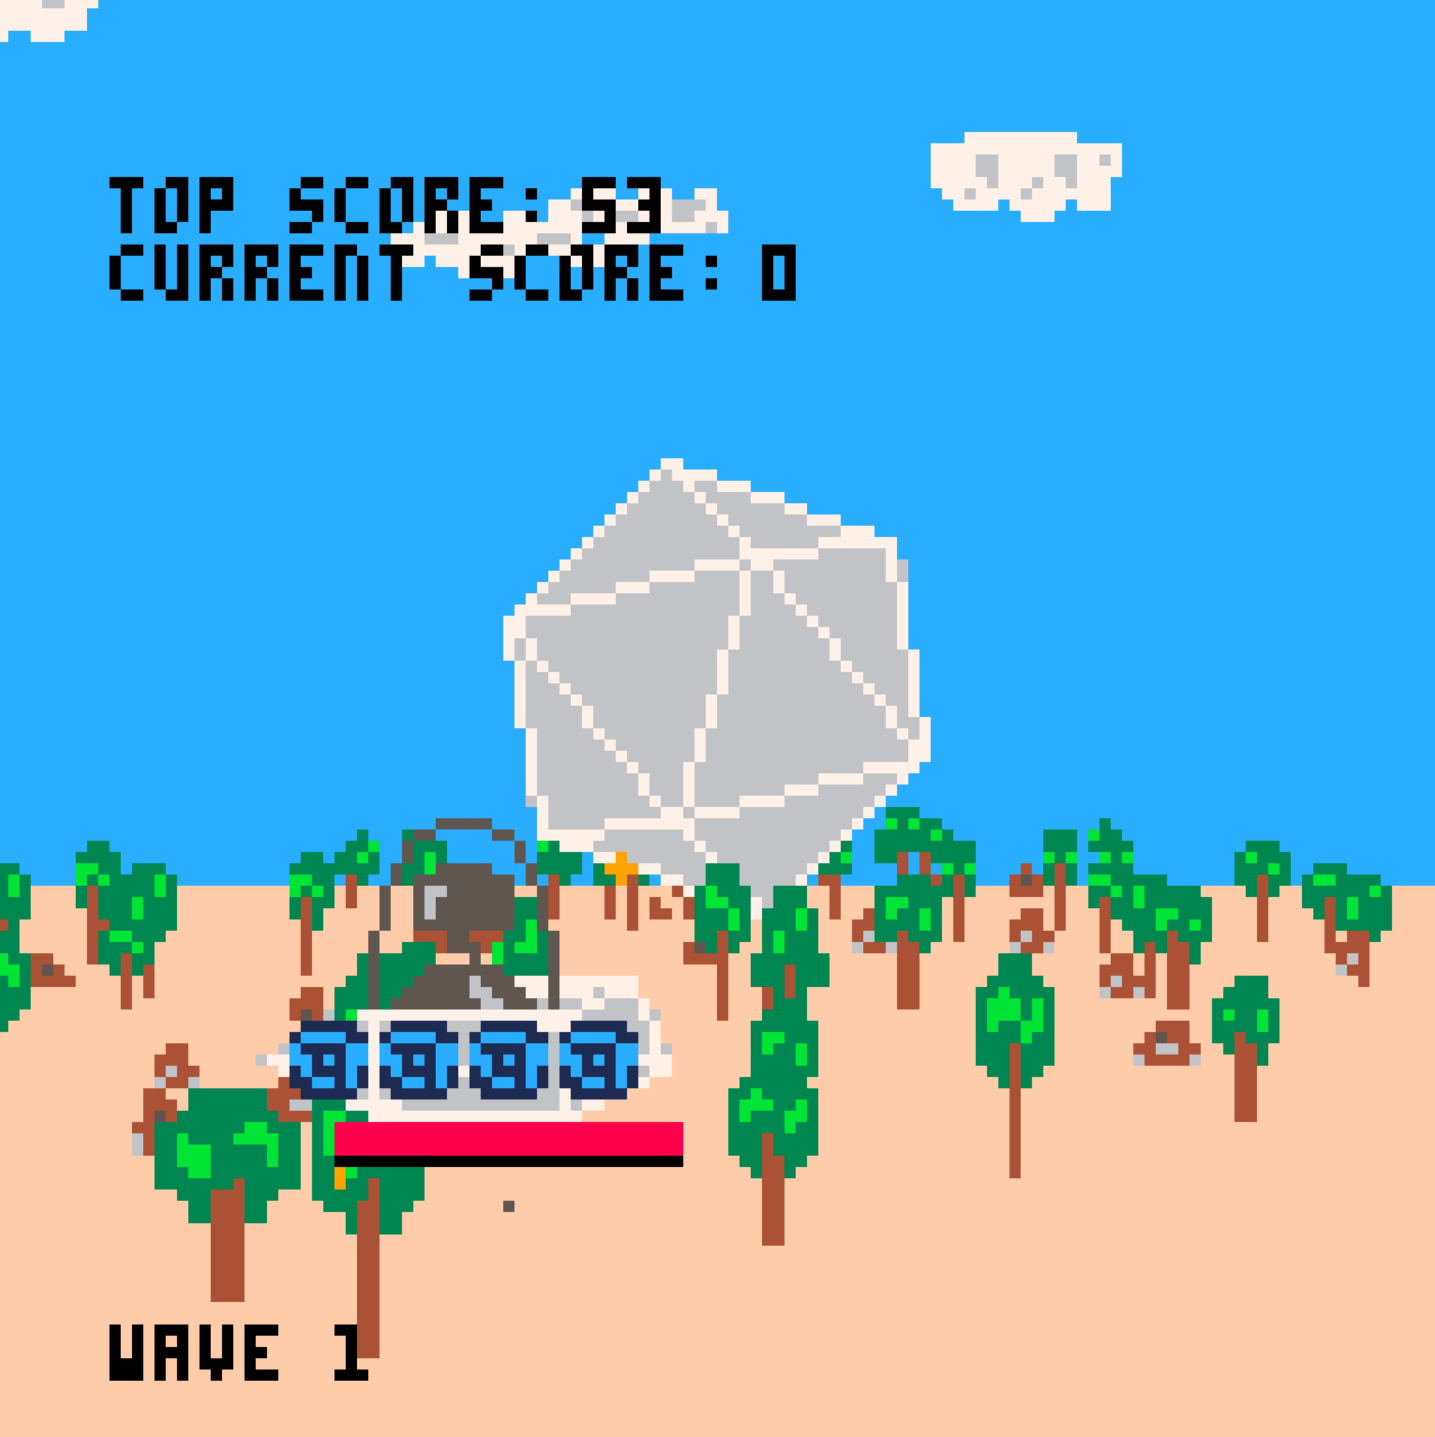
\includegraphics[width=.8\linewidth]{boss1}
  \caption{boss mode approach}
  \label{fig:bossfig1}
\end{subfigure}\hfill
\begin{subfigure}{.5\textwidth}
  \centering
  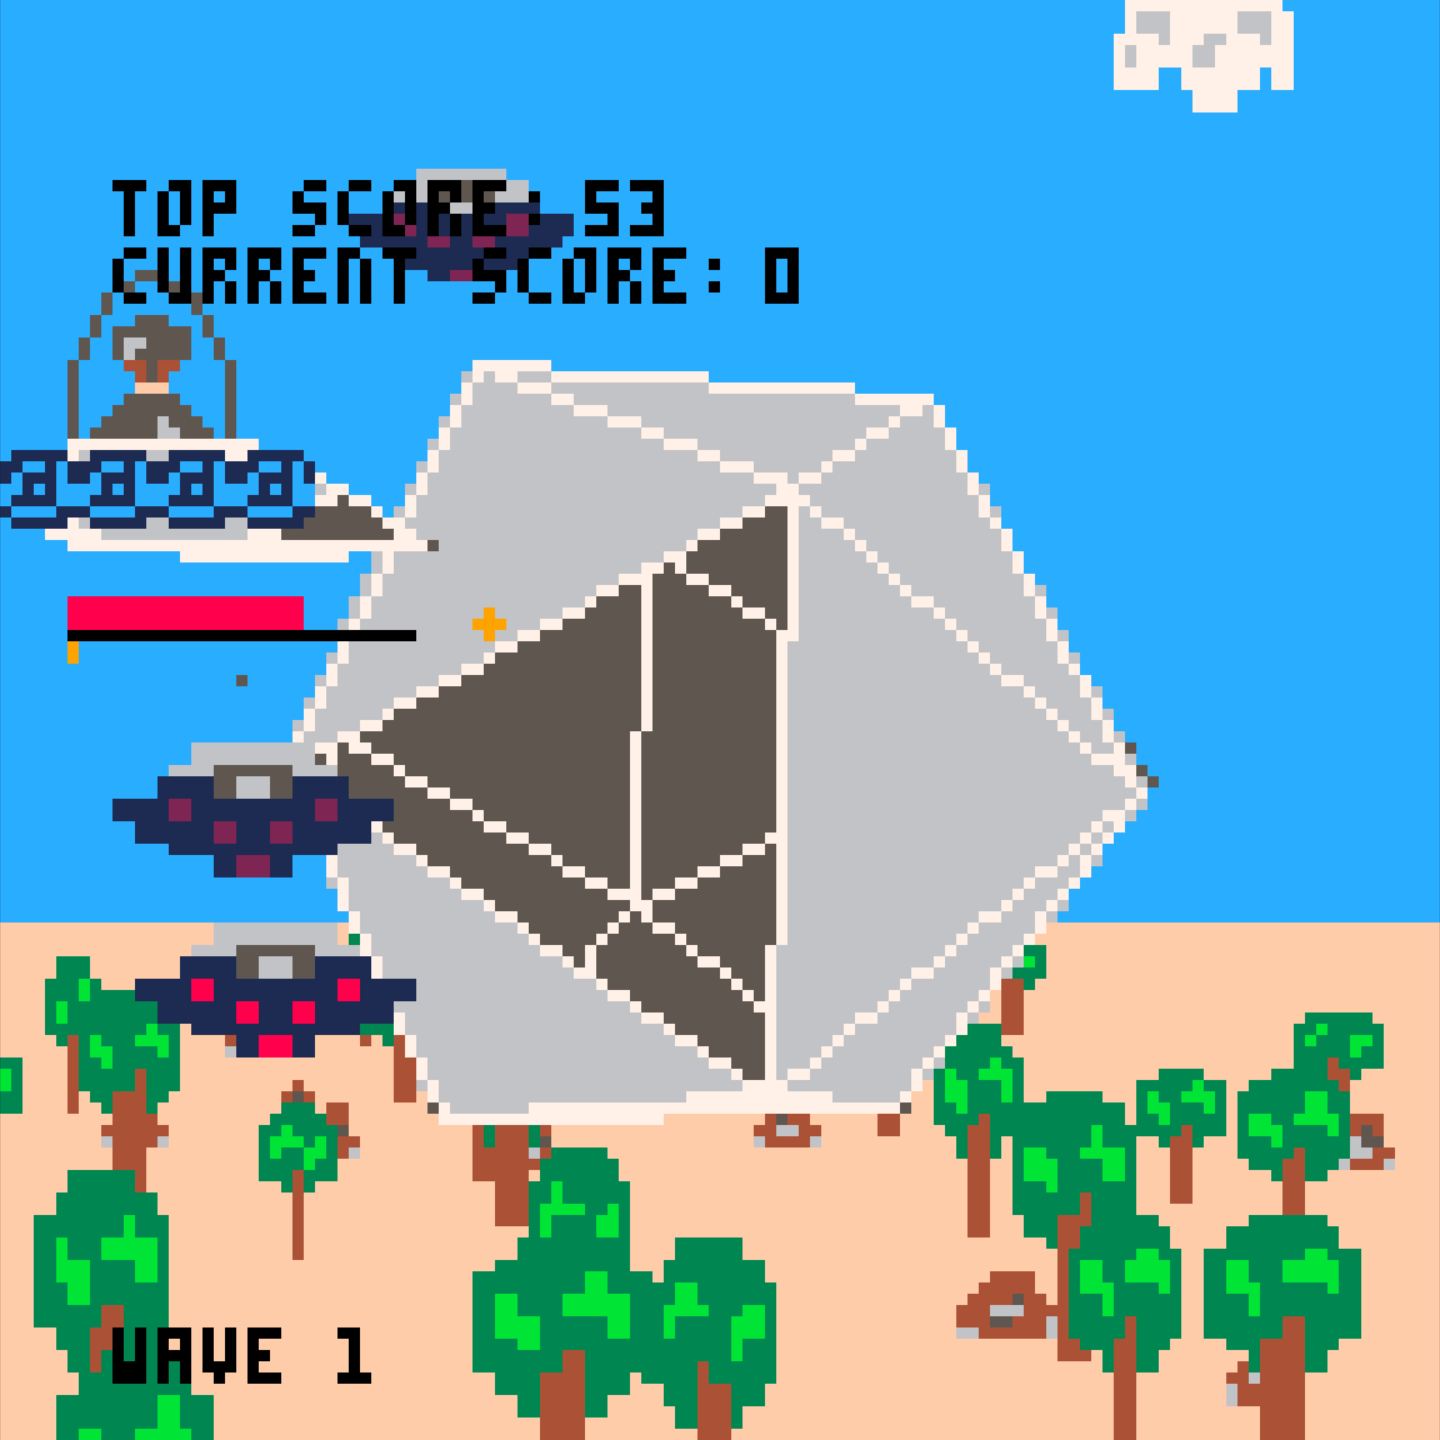
\includegraphics[width=.8\linewidth]{boss_gameplay}
  \caption{boss mode gameplay}
  \label{fig:bossfig2}
\end{subfigure}\hfill
\caption{boss mode}
\label{fig:boss}
\end{figure}

% Discuss thinking behind 3D boss design - with emphasis on opportunity to explore additional way to
% navigate 3D space with similar constraints to rail shooter genre. Compare to boss set-pieces in
% \textit{Panzer Dragoon} and \textit{Rez}.

Having implemented a core gameplay loop executing on the basic gameplay of the rail shooter genre,
development began on a climactic boss battle. Bosses in rail shooters have historically taken many
forms and suggest multiple alternative approaches - here we will briefly consider a few early
bosses from genre exemplars. 

In \textit{Space Harrier}, the player is confronted with a dragon composed of multiple
repeated sprites to represent a body, and a additional sprites to represent the head and the
point of a tail. These sprites are drawn in different orders to represent backwards and forwards
movement, and the player defeats the boss by inflicting repeated damage and reducing its size.

In \textit{Panzer Dragoon}, a more complex set piece is established in which the player (riding a 
dragon) navigates around a hostile ship in a circle - using camera controls discussed in Section
\ref{genre} and attacking turrets and other discrete parts of the ship's body.

In \textit{Rez}, the player circles around a spherical hollow shell composed of numerous discrete
faces, which they must shoot open in order to attack a point within before the shell is rebuilt.

In order to exploit built functionality for polygonal rendering and the rotation of polygonal
models - previously reserved for rendering a player ship - it was decided to opt for a boss
design more akin to \textit{Panzer Dragoon} and \textit{Rez} that worked on the principle of
circular motion around a point and the progressive destruction of a shell - combined with an 
existing enemy pattern to guard the shell.

\subsubsection*{Camera rotations in 3D space}

% Discuss the implementation of camera rotations around a point in 3D space for the
% creation of a ``boss mode'' which involves strafing around a polygonal enemy. 

In order to execute on this concept, a new camera mode had to be built for the game.
Whereas the general course of play sees the camera in a fixed position at origin, looking
along the \textit{z}-axis while enemies and geometry scroll towards it and the player
model moves in a fixed two-dimensional plane parallel to the viewport, a boss setpiece in
which the player ship strafes around a polygonal enemy required the camera to sweep in a 
circle around the boss.

Camera transformations, in this implementation, work on the principle that real camera
transformations and the application of contrary transformations on scenery objects
produce like results. As such, as illustrated in Figure \ref{fig:rotation}, camera transformations
in this mode are accomplished by transforming world scenery to simulate the movement of the camera.

In this example, to rotate objects in a scene around an arbitrary point, the objects are
translated by the inverse of the position vector of the point of rotation, rotated around
origin, and translated back by the positive position vector of the initial point.

As implemented in the game, this means that objects in the game world are rotated around
the position of the boss - at coordinates (0, 0, 5) - in the opposite direction to the
putative movement of the camera as generated by player input, in order to generate the
phenomenon of a camera sweeping through space.

\begin{figure}[h]
\begin{subfigure}{.45\textwidth}
   \centering
   \begin{tikzpicture}
      [scale = 2,
      axis/.style={-stealth},
      dot/.style= {
         draw,
         fill = black,
         circle,
         inner sep = 0pt,
         minimum size = 4pt
      },
      point/.style= {
         draw,
         fill = black,
         circle,
         inner sep = 0pt,
         minimum size = 2pt
      }]
      
      \draw[axis] (-1.25, 0) -- (1.25, 0) node[right] {$x$};
      \draw[axis] (0, -1.5) -- (0, 1.5) node[above] {$z$};

      \draw (0.5, 0.5) node[dot, label = {above:$r$}] {};
      \draw [black, ->] (0.5, 0.5) -- (0, 0);

      \draw (-0.3, 0.6) node[point, label = {above:$o_1$}] {};
      \draw [gray, ->] (-0.3, 0.6) -- (-0.8, 0.1);
      \draw (-0.8, 0.1) node[point, label = {above:$t_1$}] {};

      \draw (0.9, 0.2) node[point, label = {above:$o_2$}] {};
      \draw [gray, ->] (0.9, 0.2) -- (0.4, -0.3);
      \draw (0.4, -0.3) node[point, label = {above:$t_2$}] {};

      \draw (-0.4, -0.4) node[point, label = {above:$o_3$}] {};
      \draw [gray, ->] (-0.4, -0.4) -- (-0.9, -0.9);
      \draw (-0.9, -0.9) node[point, label = {above:$t_3$}] {};

   \end{tikzpicture}
   \caption{select point \textit{r} in 2D plane around which to rotate scene, and translate
   all objects \textit{o} by the inverse of its position vector to positions \textit{t}}
   \label{fig:rotfig1}
\end{subfigure}\hfill
\begin{subfigure}{.45\textwidth}
   \centering
   \begin{tikzpicture}
      [scale = 2,
      axis/.style={-stealth},
      dot/.style= {
         draw,
         fill = black,
         circle,
         inner sep = 0pt,
         minimum size = 4pt
      },
      point/.style= {
         draw,
         fill = black,
         circle,
         inner sep = 0pt,
         minimum size = 2pt
      }]
      \draw[axis] (-1.25, 0) -- (1.25, 0) node[right] {$x$};
      \draw[axis] (0, -1.5) -- (0, 1.5) node[above] {$z$};

      \draw (0.5, 0.5) node[dot, label = {above:$r$}] {};

      \coordinate (R) at (0.5, 0.5);

      \pgfmathsetmacro{\angle}{70}
      \pgfmathsetmacro{\tx}{-0.8}
      \pgfmathsetmacro{\ty}{0.1}
      \coordinate (t1) at (\tx, \ty);
      \pgfmathsetmacro{\rx}{\tx*cos(\angle) - \ty*sin(\angle)}
      \pgfmathsetmacro{\ry}{\tx*sin(\angle) + \ty*cos(\angle)}
      \pgfmathsetmacro{\radius}{sqrt((\tx * \tx) + (\ty * \ty))}
      \coordinate (r1) at (\rx,\ry);
      \draw (t1) node[point, label = {above:$t_1$}] {};
      \draw (r1) node[point] {};
      \begin{scope}
         \clip (-1, \ty) rectangle (0, \ry);
         \draw[densely dotted] circle(\radius);
      \end{scope}
      \draw [gray, ->] (r1) -- ($(r1)+(R)$);
      \draw ($(r1)+(R)$) node[point, label = {above:$p_1$}] {};

      \pgfmathsetmacro{\tx}{0.4}
      \pgfmathsetmacro{\ty}{-0.3}
      \coordinate (t2) at (\tx, \ty);
      \pgfmathsetmacro{\rx}{\tx*cos(\angle) - \ty*sin(\angle)}
      \pgfmathsetmacro{\ry}{\tx*sin(\angle) + \ty*cos(\angle)}
      \pgfmathsetmacro{\radius}{sqrt((\tx * \tx) + (\ty * \ty))}
      \coordinate (r2) at (\rx,\ry);
      \draw (t2) node[point, label = {above:$t_2$}] {};
      \draw (r2) node[point] {};
      \begin{scope}
         \clip (1, \ty) rectangle (0, \ry);
         \draw[densely dotted] circle(\radius);
      \end{scope}
      \draw [gray, ->] (r2) -- ($(r2)+(R)$);
      \draw ($(r2)+(R)$) node[point, label = {above:$p_2$}] {};

      \pgfmathsetmacro{\tx}{-0.9}
      \pgfmathsetmacro{\ty}{-0.9}
      \coordinate (t3) at (\tx, \ty);
      \pgfmathsetmacro{\rx}{\tx*cos(\angle) - \ty*sin(\angle)}
      \pgfmathsetmacro{\ry}{\tx*sin(\angle) + \ty*cos(\angle)}
      \pgfmathsetmacro{\radius}{sqrt((\tx * \tx) + (\ty * \ty))}
      \coordinate (r3) at (\rx,\ry);
      \draw (t3) node[point, label = {above:$t_3$}] {};
      \draw (r3) node[point] {};
      \begin{scope}
         \clip (t3) rectangle (\rx, -1.5);
         \draw[densely dotted] circle(\radius);
      \end{scope}
      \draw [gray, ->] (r3) -- ($(r3)+(R)$);
      \draw ($(r3)+(R)$) node[point, label = {above:$p_3$}] {};

   \end{tikzpicture}
   \caption{rotate translated points \textit{t} around (0, 0) and translate them again by positive
   position vector of chosen point of rotation to find final position \textit{p}}
   \label{fig:rotfig2}
\end{subfigure}\hfill
\caption{\textit{y}-axis rotation of a scene around an arbitrary point in 3D space}
\label{fig:rotation}
\end{figure}

% Highlight the implications of this change on the position and orientation of the player model,
% which can no longer exist naively in a 2D plane facing along the z-axis but which
% must now be able to exist in a rotational relationship to a focal point in the map,
% shared with the camera.

This change also forced reconsideration of how the position of the player is defined
in the game world, and associated issues such as direction of fire. Whereas the position
of the player ship had previously been defined as a point in 3D space confined to a 2D
plane parallel to the camera viewport, free-firing projectiles directly down the \textit{z}-axis,
strafing motion around a stationary boss setpiece required the position of the ship to instead
be defined by an angle around a unit circle.

Two alternative approaches to free-firing under this new approach were considered. Firstly,
the technically correct approach, would see the ship firing directly forward as it faced - with
the unfortunate implication that all shots would ultimately travel through the centre of
rotation, and thus cause undue constraint on player action. The alternative, which was adopted,
saw the ship maintain its freedom to fire from arbitrary points on a 2D plane by directing
bullets down the direction faced by the camera rather than the player ship - a trade-off
that favoured game feel over accurate simulation.

% Discuss the relationship between in-frame player movement,
% the implied field of view of a 1x1 canvas at single unit distance from pinhole, and
% camera rotation around a point. Discuss the per-object rotations required to execute
% such camera movements, density of spawned scenery, and concerns around computational
% load.

\subsubsection*{Ray-triangle collision with the Möller–Trumbore algorithm}

% Discuss the need for more complex ray-triangle intersection computations to effectively
% test for collisions around the boss enemy, since the intended design requires per-face
% collision detection on a regular icosahedron whose faces cannot be satisfactorily
% split into non-overlapping cuboid bounding volumes that adequately approximate
% collisions.

Because the hollow boss enemy shell is composed of twenty triangles forming a regular icosahedron,
and each of the individual triangles needed to be individually destructible, the simple hitbox
approach outlined in Section \ref{conversion} was not sufficient to correctly model the intended
behaviour of the game. As such a more complex collision detection algorithm was required, capable
of handling collisions between moving points (in-game projectiles) and triangles in 3D space.

The Möller–Trumbore algorithm for ray-triangle intersections was selected, as an efficient and well
understood approach to solving this issue which does not require prior preparation of the triangles
to be inspected (and thus avoids the token overhead an alternative approach may require).
The implementation of this algorithm fit comfortably in the frame budget of the game, despite
several calls to relatively expensive linear algebraic functions.

The implementation of the collision detection algorithm is excerted in Figure \ref{fig:codemoller}, and is
directly adapted from the C++ published by Möller and Trumbore in \cite{möller–trumbore}.

\begin{figure}[h]
   \begin{lstlisting}
bullet_triangle_intersect = function(self, bullet, triangle)

   epsilon = 0.0001

   vert0 = self.current_vertices[triangle[1]]
   vert1 = self.current_vertices[triangle[2]]
   vert2 = self.current_vertices[triangle[3]]

   edge1 = subtract(vert1, vert0)
   edge2 = subtract(vert2, vert0)

   pvec = cross_product({bullet.x_increment, bullet.y_increment, bullet.z_increment}, edge2)

   det = dot_product(edge1, pvec)

   -- only use non-culling branch from paper, since boss shell is hollow and can be shot through
   if det > -epsilon and det < epsilon then return false end

   inv_det = 1 / det

   tvec = subtract({bullet.x, bullet.y, bullet.z}, vert0)
   u = dot_product(tvec, pvec) * inv_det
   if (u < 0 or u > 1) then return false end

   qvec = cross_product(tvec, edge1)
   v = dot_product({bullet.x_increment, bullet.y_increment, bullet.z_increment}, qvec) * inv_det
   if (v < 0 or u + v > 1) then return false end

   t = dot_product(edge2, qvec) * inv_det

   if t <= 1 then return true else return false end

end
   \end{lstlisting}
   \caption{Möller–Trumbore algorithm for ray-triangle intersections}
   \label{fig:codemoller}
\end{figure}

One limitation of this approach is that projectiles are modelled as points in space rather than
objects with volume, which is contrary to their handling in other game situations, but this
inconsistency was accepted on the previously mentioned principle of ``if it feels right, it is
right'', which is one of the advantages of working in non-critical real time applications -
allowing us to eschew the additional overhead of performing this calculation for the eight vertices
of a cuboid bounding volume, or implementing a more bespoke calculation that accurately tests for
the collision of a triangle with any points on the surface of a sphere.

\section{Results and evaluation}

\subsection{Testing feedback}
Two forms of user evaluation were performed in the course of development. In addition to the
quantitative task load evaluation performed to evaluate the effectiveness of different kinds
of enemy speed scaling, discussed in Section \ref{update}, the game was also subject to
less formal qualitative user testing, conducted through relatively unstructured think aloud sessions.

As discussed in Section \ref{draw}, the design of the Heads Up Display - giving the user information
about their health, cooldown status, and lock-on limit - was redesigned to answer feedback that
the information was widely ignored in favour of focus on the core shooting action of the game. As
such, it was repositioned to follow the player ship model and provide easier to reference information
about the current state of the run.

The initial round design of pick-up sprites was also a source of confusion for players, who would
avoid them between waves in the belief that they were actually projectiles - a confusion caused by
the red and orange colouring shared with enemy projectiles in the rest of the game, and their round
appearance. As such they were redesigned to have square shapes, and recoloured to avoid conflicts with
hostile projectiles.

One think aloud tester also questioned the purpose of the game and suggested the inclusion of an explicit
narrative element - this was useful feedback and could form the basis of additional work, but was not
prioritised as essential work for the project prior to submission.

There was also positive feedback from these sessions too. Users uniformly expressed comfort with
interpeting depth in the game, despite its low resolution and use of 2D sprites. They also
considered hit detection fair, and did not complain about missed shots caused by inconsistencies
in game code.

The game could certainly benefit from additional testing, and ideas for additional
tests have been suggested in Section \ref{additionaltests}.

\subsection{Pitfalls of paper prototyping for 3D projects}\label{prototypepitfalls}

The paper prototype did succeed in distilling the core aim, target, and shoot mechanics
of the core game loop, and various aspects of the design that were jettisoned - such as
the upright player sprite and the faked scrolling of the ground - were largely cosmetic.

But while it distilled the core elements of the game successfully, there was a sense in
which the prototype was also unhelpful. Because of the flat and fundamentally two-dimensional
nature of a rudimentary paper prototype, the developer is encouraged to consider the
problems posed by the project in a two-dimensional way. As such, much of the initial prototyping
phase was not as productive as it might otherwise be, since the underlying thinking about
projecting and operating with regard to 3D space was elided.

Although it had some utility in terms of encouraging thinking about game feel and anticipating
design concerns that were not significantly impacted by the 3D environment - for example, about
the introduction of limits to the lock-on capability - it also spent up a lot of development time
building functionality that ultimately had to be fundamentally rethought and reimplemented to
accomodate the 3D ambitions of the project.

\subsection{Artificial limits imposed by featly to platform ethos}

An early commitment to the underlying ethos of PICO-8 led to a misguided interest in producing
a piece of software that was bound by the single-cart token limit imposed by the system, despite
the fact that multicart games are a known approach and daisy-chaining carts together is a fairly
trivial feature provided by the system and supported in deployment.

As such, while scope control was an important part of the project, it could be said that the
scope was artificially narrowed to what could realistically (but not actually) fit on a single cart.

Once the move to a multicart design had been forced by a late encounter with PICO-8's token limit,
it became obvious that more could be done with the game using existing functionality to build a richer
and more varied gameplay experience. Those additional modes will be discussed in Section \ref{furtherwork}

\section{Further work}\label{furtherwork}

\subsection{Additional testing and mechanical pivots}\label{additionaltests}

Two areas of the game design would clearly benefit from additional testing.

One persistent issue revealed in user testing, that was not adequately handled at the completion of
the project as it exists, was player disinterest in using the given lock-on functionality.

Resolution of this design issue could be informed by a round of additional testing, presenting
alternative mechanics to the lock-on as currently implemented.

One approach, which has the downside
of reducing player agency, is to simply make lock-on mandatory for firing - which is the approach
taken in \textit{Rez}, presumably so that the developer can exercise greater control over the timing
of firing events and better synchronise diagetic sound to the game's electronic score.

An alternative approach would be to jettison the lock-on mechanic entirely, in the face of
player disinterest, and replace it with an alternative behaviour for holding to fire - one
suggestion, volunteered by a think-aloud tester, was to replace this mechanic with a weapon
charging mechanic, allowing players to fire off more or less powerful free shots by holding
the input for more or less time.

This would pose the additional problem of either adding
additional information to the HUD in order to illustrate charge level, or else to rely on
player intuition and risk creating a false feeling of uncertainty. It would also require
the health of enemies to be rethought - they are currently killed on impact with
a player projectile, whereas a more complex approach to health would need to be devised
to accomodate player projectiles of varied strength.

A second subject for testing would be the boss encounter in its entirety. Because of its late
development in the project, it was not properly tested either in qualitative think aloud sessions
or in quantitative evaluation, and thus it has not been possible to effectively evaluate it 
in use. As such, it is not known if the encounter places excessive load on the player by 
combining a strafing chase for a weak surface with free firing and hostile enemy targets, and
if this load can be alleviated by tweaking levels of speed or enemy density.

Likewise, it is not known if players will intuitively understand how the boss works and what
they are expected to do, or - if they do - whether they understand that the boss rotates in a 
predictable pattern that allows you to efficiently take shots by remaining in the a position
that sees the weak face routinely pass.

\subsection{Additional mode development}

Following the switch to a multicart design late in the project, one obvious path for future
development is the exploration of additional gameplay modes that were originally considered
out of scope due to the token limit constraint that exists with single cart PICO-8 games.
Here I will briefly discuss some game modes that could be straightforwardly implemented
given functionality that has already been built to rotate our camera around arbitrary
points in 3D space.

The first such mode would be a side-on mode in which the player continues to move forward
through space but in which the camera now views the player side-on - changing player directional
inputs from controlling direction in the \textit{x} and \textit{y} planes and instead giving
limited control along \textit{z} and \textit{y}.

This player movement and camera set-up would be combined with an enemy approach along the
\textit{z}-axis, on a parallel plane further along the \textit{x}-axis, resulting in gameplay
broadly similiar to that found in the existing game - except with continuous motion now
simulated along the screen rather than down it.

This is broadly in line with the approach taken in \textit{Rez}, where scripted camera movements
result in side-along gameplay and occasional enemy movement from the rear. Such gameplay also
exists in \textit{Panzer Dragoon}, although it is initiated by the player - who can rotate the
camera to four cardinal positions around the dragon using the Sega Saturn's shoulder inputs.

Such an additional mode would highlight the three-dimensional nature of the game world and
create a dynamic alternative to repeated enemy waves using the same camera set-up.

The second such mode, closely related to the first, would be a shoot 'em up mode where the player
and enemies all exist on the same plane parallel to the camera, and the player evades and fires shots
directly along the relative $x$-axis of our screen - as is the case in a huge and persistently popular
genre of game in its own right. Unlike the side-on chase mode outlined above, the implementation of
a satisfying shoot 'em up mode would require extensive design thinking, and investigation of the
known conventions of that genre in its own right.

\subsection{Change of technology}\label{engines}

As outlined in Section \ref{pico}, PICO-8 is an excellent prototyping tool. But it is inherently
limited, and one obvious course of future work would be to translate the game to more robust technology
and explore the creative possibilities unlocked by a less constrained development environment - most
notabily in graphical effects and in sound synchronisation.

Switching to either an off-the-shelf game engine such as Unreal, Unity, or Godot, or to a minimal but
less built out game development library like Raylib, would allow the development of a more sophisticated
game experience that advances beyond the borders imposed by PICO-8.

Most obviously such a change of technology would allow the creation of a full polygonal game world,
in which objects can be comfortably displayed at smaller scales on a more detailed pixel grid, and
shaded appropriately by a colour palette that contains more than 16 discontinuous colours.

It would also offer the opportunity to get more creative with the sound design of the game. At present,
the game implements a small set of sound effects to represent projectile firing, projectile collisions,
the acquisition of enemy targets and power-ups, and the fan-like motion of drone blades passing the player.
But no effort has been made to implement a musical soundtrack - both because of the general musical illiteracy
of the developer, and also the extreme constraints placed on PICO-8 by its four-channel blip-based
music engine.

One of the most interesting possibilities of the rail shooter genre, touched on by \textit{Rez}, is the ability
to effectively leverage the highly scripted nature of the game to produce stunning synchronisation effects.
In the case of \textit{Rez}, those effects simulate a kind of player participation in the game's score - with
projectiles initiated by the player colliding with enemies and creating beats in a cleverly synchronised way.

One alternative approach that could be taken, leveraging the genre's potential for synchronisation, would be to
instead more closely marry the movement of enemy units with a rich, potentially balletic score. Such an exercise
would be futile in PICO-8, both because of limitations on the sound engine preventing the creation of satisfying
polyphonic music, and because data constraints - even in a heavily daisy-chained game - limiting the ability to
precisely specify enemy movement beyond simple rule following.

\section{Conclusion}
At the end of this project, a complete slice of gameplay has been built - including
a core rail shooter gameplay loop featuring a variety of enemy patterns, alternative free
firing and lock-on firing modes, a boss encounter set piece, 
accurate 3D perspective projection for both sprites and polygonal models,
and real-time collision detection for cuboid bounding volumes and
more complex ray-triangle intersections.

Development has been constrained (as intended due to project scope) by the known
system constraints of our chosen technology, the ``fantasy console'' PICO-8. However,
we have also seen how it was ultimately constrained to an unnecessary degree by
an arbitrary sense of fealty to the technology's founding ethos despite known
mitigations for that particular constraint - namely, the constraint imposed by
per-cart token limits and the ability to work around them by daisy-chaining
carts containing different gameplay sections.

Possibilities for future development of the project, built on top of the successful
creation of a playable slice, have been outlined - up to and including a significant
change in technology to pursue more ambitious designs.

\printbibliography

\end{document}